% =====================================================================
%  MANUAL DE SOBREVIVENCIA DO CIENTISTA SOCIAL COM IA
%  Manual pratico, complementar ao Mini Curso do CEM
%  Redesenho: identidade amigavel/ludica, herdando a paleta e a marca do CEM
% =====================================================================
\documentclass[11pt,a4paper]{article}
\usepackage{fontspec}
% Nota: pacote de idioma (babel/polyglossia) para pt-BR indisponivel neste
% ambiente de compilacao (faltam os arquivos de idioma e hifenizacao). O
% documento usa aspas e pontuacao digitadas manualmente, entao compila sem
% ele; a unica perda e a hifenizacao automatica de portugues nas quebras de linha.
\usepackage{tgschola}
\usepackage{microtype}
\usepackage{amssymb}
\usepackage[a4paper,top=1.7cm,bottom=1.9cm,left=1.9cm,right=1.9cm]{geometry}
\usepackage[table,dvipsnames]{xcolor}

% ---------- Paleta: azuis institucionais do CEM + acentos ludicos ----------
\definecolor{azulUNI}{RGB}{31,78,121}
\definecolor{azulUNIclaro}{RGB}{68,114,150}
\definecolor{azulUNIsuave}{RGB}{223,232,242}
\definecolor{laranjaDestaque}{RGB}{202,96,28}
\definecolor{amareloSol}{RGB}{225,163,45}
\definecolor{verdeCodigo}{RGB}{0,110,80}
\definecolor{cinzaCodigo}{RGB}{246,246,244}
\definecolor{cinzaSaida}{RGB}{238,241,244}
\definecolor{cinzaescuro}{RGB}{58,58,58}

% ---------- Tipografia: Poppins (titulos) + TeX Gyre Schola (corpo) ----------
\newfontfamily\poppins{Poppins}
\newfontfamily\poppinsmed{Poppins Medium}

\usepackage{tikz}
\usetikzlibrary{shapes.geometric,arrows.meta,positioning,calc,fit,backgrounds}
\usepackage{tcolorbox}
\tcbuselibrary{skins,breakable}
\usepackage{booktabs}
\usepackage{array}
\usepackage{enumitem}
\usepackage{titlesec}
\usepackage{multicol}
\usepackage{fancyhdr}
\usepackage{graphicx}
\usepackage{hyperref}
\hypersetup{colorlinks=true,linkcolor=azulUNI,citecolor=laranjaDestaque,urlcolor=azulUNI}
\usepackage{xurl}
\usepackage{listings}
\lstset{
  basicstyle=\ttfamily\scriptsize,
  backgroundcolor=\color{cinzaCodigo},
  frame=single,
  rulecolor=\color{azulUNIclaro},
  framerule=0.5pt,
  breaklines=true,
  breakatwhitespace=true,
  columns=flexible,
  keepspaces=true,
  showstringspaces=false,
  xleftmargin=4pt, xrightmargin=4pt, aboveskip=4pt, belowskip=4pt,
  extendedchars=true, literate=
    {á}{{\'a}}1 {à}{{\`a}}1 {â}{{\^a}}1 {ã}{{\~a}}1
    {é}{{\'e}}1 {ê}{{\^e}}1
    {í}{{\'i}}1
    {ó}{{\'o}}1 {ô}{{\^o}}1 {õ}{{\~o}}1
    {ú}{{\'u}}1 {ü}{{\"u}}1
    {ç}{{\c c}}1
    {Á}{{\'A}}1 {À}{{\`A}}1 {Â}{{\^A}}1 {Ã}{{\~A}}1
    {É}{{\'E}}1 {Ê}{{\^E}}1
    {Í}{{\'I}}1
    {Ó}{{\'O}}1 {Ô}{{\^O}}1 {Õ}{{\~O}}1
    {Ú}{{\'U}}1 {Ü}{{\"U}}1
    {Ç}{{\c C}}1
}
\setlength{\parindent}{0pt}
\setlength{\parskip}{4pt}

% =====================================================================
%  ICONES (traco fino, desenhados em TikZ, coerentes com a marca do CEM)
% =====================================================================
\newcommand{\iconBulb}[1]{%
  \begin{tikzpicture}[baseline=-0.55ex]
    \draw[#1,line width=1pt,line cap=round] (0,0.03) circle (0.13);
    \draw[#1,line width=1pt] (-0.05,-0.1) -- (0.05,-0.1);
    \draw[#1,line width=1pt] (-0.04,-0.15) -- (0.04,-0.15);
    \draw[#1,line width=0.8pt] (0,-0.1) -- (0,-0.01);
  \end{tikzpicture}}
\newcommand{\iconWarn}[1]{%
  \begin{tikzpicture}[baseline=-0.55ex]
    \draw[#1,line width=1pt,line join=round] (-0.15,-0.12) -- (0.15,-0.12) -- (0,0.16) -- cycle;
    \draw[#1,line width=1pt] (0,-0.03) -- (0,0.04);
    \fill[#1] (0,-0.08) circle (0.015);
  \end{tikzpicture}}
\newcommand{\iconBookmark}[1]{%
  \begin{tikzpicture}[baseline=-0.55ex]
    \draw[#1,line width=1pt,line join=round] (-0.11,0.15) -- (0.11,0.15) -- (0.11,-0.15) -- (0,-0.03) -- (-0.11,-0.15) -- cycle;
  \end{tikzpicture}}
\newcommand{\iconCode}[1]{%
  \begin{tikzpicture}[baseline=-0.55ex]
    \draw[#1,line width=1.1pt,line cap=round,line join=round] (-0.03,0.13) -- (-0.16,0) -- (-0.03,-0.13);
    \draw[#1,line width=1.1pt,line cap=round,line join=round] (0.03,0.13) -- (0.16,0) -- (0.03,-0.13);
  \end{tikzpicture}}
\newcommand{\iconCheck}[1]{%
  \begin{tikzpicture}[baseline=-0.55ex]
    \draw[#1,rounded corners=1pt,line width=1pt] (-0.15,-0.15) rectangle (0.15,0.15);
    \draw[#1,line width=1.1pt,line cap=round,line join=round] (-0.08,0) -- (-0.02,-0.07) -- (0.09,0.09);
  \end{tikzpicture}}
\newcommand{\iconCompass}[1]{%
  \begin{tikzpicture}[baseline=-0.55ex]
    \draw[#1,line width=1pt] (0,0) circle (0.16);
    \draw[#1,line width=0.9pt,line join=round,fill=#1] (0,0.09) -- (0.045,-0.02) -- (0,-0.09) -- (-0.045,-0.02) -- cycle;
  \end{tikzpicture}}

% ---------- distintivo circular numerado (secoes) ----------
\newcommand{\secbadge}[1]{\tikz[baseline=-0.8ex]{\node[circle,fill=azulUNI,text=white,font=\poppins\bfseries,inner sep=0pt,minimum size=0.92cm] {#1};}}
% ---------- distintivo em pilula (modelos de prompt numerados) ----------
\newcommand{\pillbadge}[2]{\tikz[baseline=-0.75ex]{\node[circle,fill=#2,text=white,font=\poppins\bfseries\small,inner sep=0pt,minimum size=0.72cm] {#1};}}

% =====================================================================
%  DISPERSAO DE PONTOS (motivo visual herdado da marca do CEM)
% =====================================================================
\colorlet{dotcolor0}{azulUNI}
\colorlet{dotcolor1}{cinzaescuro}
\colorlet{dotcolor2}{azulUNIclaro}
\newcommand{\dotcluster}[3]{%
\pgfmathsetseed{11}
\foreach \i in {1,...,#1}{
  \pgfmathsetmacro{\x}{rnd*#2}
  \pgfmathsetmacro{\y}{rnd*#3}
  \pgfmathsetmacro{\r}{0.02+0.05*rnd}
  \pgfmathtruncatemacro{\m}{mod(\i,3)}
  \fill[dotcolor\m] (\x,\y) circle (\r);
}}

% ---------- Titulos de secao: distintivo numerado + Poppins ----------
\titleformat{\section}
  {\normalfont\Large\poppins\bfseries\color{azulUNI}}
  {\secbadge{\thesection}}
  {10pt}
  {}
  [{\vspace{3pt}\color{azulUNIclaro}\titlerule[1.2pt]}]
\titleformat{\subsection}{\normalfont\large\poppins\bfseries\color{azulUNI}}{\thesubsection}{6pt}{}
\titlespacing*{\section}{0pt}{16pt}{8pt}
\titlespacing*{\subsection}{0pt}{10pt}{4pt}

% ---------- Cabecalho e rodape ----------
\pagestyle{fancy}
\setlength{\headheight}{22pt}
\fancyhf{}
\renewcommand{\headrulewidth}{0.6pt}
\renewcommand{\headrule}{\color{azulUNIclaro}\hrule width\headwidth height\headrulewidth}
\fancyhead[L]{\raisebox{-0.19cm}{
\includegraphics[height=0.46cm]{assets/cem_mark.png}}\ \ \poppinsmed\small\color{cinzaescuro} Manual de Sobrevivência do Cientista Social com IA}
\fancyhead[R]{\poppinsmed\small\color{cinzaescuro} Minicurso do CEM $\bullet$ 2026}
\fancyfoot[C]{\tikz[baseline=-0.65ex]{\node[circle,fill=azulUNIclaro,text=white,font=\poppins\bfseries\small,inner sep=0pt,minimum size=0.55cm]{\thepage};}}

% ---------- Caixas ----------
\newtcolorbox{regra}[1][]{enhanced,colback=azulUNI,colframe=azulUNI,coltext=white,
  fonttitle=\poppins\bfseries,boxrule=0pt,arc=10pt,left=14pt,right=14pt,top=9pt,bottom=9pt,
  drop shadow=black!35,#1}
\newtcolorbox{dica}[1][]{colback=cinzaSaida,colframe=verdeCodigo,coltitle=white,
  colbacktitle=verdeCodigo,fonttitle=\poppins\bfseries,title={\iconBulb{white}\ \ Dica},boxrule=0.7pt,arc=3pt,
  left=7pt,right=7pt,top=5pt,bottom=5pt,#1}
\newtcolorbox{atencao}[1][]{colback=cinzaSaida,colframe=laranjaDestaque,coltitle=white,
  colbacktitle=laranjaDestaque,fonttitle=\poppins\bfseries,title={\iconWarn{white}\ \ Atenção},boxrule=0.7pt,arc=3pt,
  left=7pt,right=7pt,top=5pt,bottom=5pt,#1}
\newtcolorbox{leitura}[1][]{colback=cinzaSaida,colframe=azulUNI,coltitle=white,
  colbacktitle=azulUNI,fonttitle=\poppins\bfseries,boxrule=0.7pt,arc=3pt,
  left=7pt,right=7pt,top=5pt,bottom=5pt,#1}
\newtcolorbox{modelo}[3][]{colback=cinzaCodigo,colframe=azulUNIclaro,coltitle=white,
  colbacktitle=azulUNIclaro,fonttitle=\poppins\bfseries,
  title={\raisebox{-0.13cm}{\pillbadge{#2}{azulUNI}}\ \ \iconCode{white}\ \ #3},
  boxrule=0.7pt,arc=3pt,left=7pt,right=7pt,top=6pt,bottom=6pt,#1}
\newtcolorbox{checklist}[3][]{colback=white,colframe=#2,coltitle=white,
  colbacktitle=#2,fonttitle=\poppins\bfseries,title={\iconCheck{white}\ \ #3},
  boxrule=0.8pt,arc=4pt,breakable,left=9pt,right=9pt,top=7pt,bottom=7pt,#1}
\newcommand{\checkboxicon}[1]{\tikz[baseline=-0.05cm]{\node[draw=#1,thick,rounded corners=1.2pt,minimum width=0.34cm,minimum height=0.34cm,inner sep=0pt]{};}}
\newcommand{\itemcheck}[2][azulUNI]{\item[\checkboxicon{#1}] #2}

% ---------- referencia comentada + selo de nivel (bibliografia) ----------
\newcommand{\refc}[2]{\item #1\\{\footnotesize\color{cinzaescuro}\textit{#2}}}
\newcommand{\nivelbasico}{\hfill\colorbox{verdeCodigo}{\color{white}\scriptsize\poppinsmed\textbf{~BÁSICO~}}}
\newcommand{\nivelinterm}{\hfill\colorbox{amareloSol}{\color{black}\scriptsize\poppinsmed\textbf{~INTERMEDIÁRIO~}}}
\newcommand{\nivelavancado}{\hfill\colorbox{laranjaDestaque}{\color{white}\scriptsize\poppinsmed\textbf{~AVANÇADO~}}}

\setlist{nosep,leftmargin=1.2em}

\begin{document}

% =====================================================================
%  CAPA
% =====================================================================
\thispagestyle{empty}
\vspace*{\fill}

\begin{center}
\begin{tikzpicture}
\node[anchor=north west, inner sep=0pt] at (-1.4,0) {\begin{tikzpicture}\dotcluster{26}{2.3}{1.05}\end{tikzpicture}};
\node[anchor=north east, inner sep=0pt] at (7.6,0) {
\begin{tikzpicture}[xscale=-1]\dotcluster{26}{2.3}{1.05}\end{tikzpicture}};
\node at (3.1,-0.6) {
\includegraphics[width=3.6cm]{assets/cem_logo_trim.png}};
\end{tikzpicture}

\vspace{6pt}
{\poppins\bfseries\footnotesize\color{laranjaDestaque} MINICURSO DO CEM}

\vspace{10pt}
{\poppins\Huge\bfseries\color{azulUNI} Manual de Sobrevivência}\\[5pt]
{\poppins\LARGE\bfseries\color{laranjaDestaque} do Cientista Social com IA}\\[9pt]
{\poppinsmed\large\color{cinzaescuro} Manual prático para o uso de ferramentas de IA para Cientistas Sociais}
\end{center}

\vfill

\begin{center}
{\poppinsmed\large\color{cinzaescuro} Anderson Henrique}\\[4pt]
{\poppinsmed\small\color{cinzaescuro} 1ª edição --- 2026}
\end{center}

\vspace{14pt}
\begin{regra}
  \poppins\large\centering
  Verificar toda referência $\;\bullet\;$ Declarar todo uso $\;\bullet\;$ Nunca terceirizar o juízo
\end{regra}
\vspace*{1.1cm}

\clearpage
% =====================================================================
%  FOLHA DE ROSTO / FICHA TECNICA
% =====================================================================
\thispagestyle{empty}

\vspace*{0.3cm}
\begin{tcolorbox}[colback=azulUNIsuave!45,colframe=azulUNI,boxrule=0.8pt,arc=5pt,left=14pt,right=14pt,top=11pt,bottom=11pt]
{\poppins\Large\bfseries\color{azulUNI} Orientações de como usar este manual}\\[7pt]
\large
Este não é um resumo das aulas. É um manual para consultar \textbf{quando você, de fato, for usar a IA} para uma tarefa de pesquisa, ensino ou escrita. Volte a ele sempre que precisar decidir se a IA irá te ajudar na realização da tarefa e de que forma ela será usada.

\vspace{7pt}
As orientações estão organizadas conforme a ordem e a frequência em que as dúvidas costumam aparecer nas aulas e minicursos, considerando: o vocabulário, a escolha adequada da ferramenta e do esforço certos, os modelos de prompt prontos, até como emitir a declaração de uso no seu manuscrito.
\end{tcolorbox}

\vspace{14pt}
\begin{tcolorbox}[colback=cinzaSaida,colframe=verdeCodigo,boxrule=0.8pt,arc=5pt,left=14pt,right=14pt,top=10pt,bottom=10pt]
{\poppins\bfseries\small\color{verdeCodigo} AGRADECIMENTOS}\\[6pt]
\small
Agradecemos aos comentários e às sugestões dos professores Janedalva Gondim (Univasf), Marcílio Brandão (Univasf), Dalson Figueiredo Filho (UFPE) e Pedro Palotti (IPEA) para a edição final deste manual.
\end{tcolorbox}

\vspace{18pt}
\begin{tcolorbox}[colback=white,colframe=cinzaescuro,boxrule=0.8pt,arc=5pt,left=14pt,right=14pt,top=10pt,bottom=10pt]
{\poppins\bfseries\small\color{cinzaescuro} FICHA TÉCNICA}\\[7pt]
\small
\renewcommand{\arraystretch}{1.5}
\begin{tabular}{@{}p{2.6cm}p{12.9cm}@{}}
\textbf{\poppinsmed\color{azulUNI}Título} & Manual de Sobrevivência do Cientista Social com IA: manual prático complementar ao minicurso \textit{Introdução à Inteligência Artificial Generativa nas Ciências Sociais} \\
\textbf{\poppinsmed\color{azulUNI}Autor} & Anderson Henrique \\
\textbf{\poppinsmed\color{azulUNI}Objetivo} & Pensado para auxiliar estudantes, professores ou cientistas sociais a usarem a IA em suas atividades de pesquisa, ensino e escrita. \\
\textbf{\poppinsmed\color{azulUNI}Site} & \url{www.ahenriquecp.com} \\
\textbf{\poppinsmed\color{azulUNI}Contato} & andersonheri@gmail.com \\
\textbf{\poppinsmed\color{azulUNI}Financiamento} & Fundação de Amparo à Pesquisa do Estado de São Paulo (FAPESP), processo 2025/15250-0 \\
\textbf{\poppinsmed\color{azulUNI}Edição} & 1ª edição, 2026 \\
\textbf{\poppinsmed\color{azulUNI}Como citar} & HENRIQUE, Anderson. \textit{Manual de sobrevivência do cientista social com IA}: manual prático. São Paulo: Centro de Estudos da Metrópole (CEM/USP), 2026. DOI: 10.5281/zenodo.21982080. \\
\textbf{\poppinsmed\color{azulUNI}Uso e licença} & Material de uso educacional. Reprodução e compartilhamento livres para fins não comerciais, desde que citada a fonte. \\
\end{tabular}
\end{tcolorbox}

\vspace{18pt}
\begin{tcolorbox}[colback=azulUNIsuave!45,colframe=azulUNI,boxrule=0.8pt,arc=5pt,left=14pt,right=14pt,top=11pt,bottom=11pt]
{\poppins\bfseries\small\color{azulUNI} DECLARAÇÃO DE USO DE INTELIGÊNCIA ARTIFICIAL}\\[6pt]
\small
Este trabalho utilizou Claude Sonnet 4.5 (Anthropic) entre julho e agosto de 2026. Uso que moldou diretamente o conteúdo: edição e depuração do código-fonte em LaTeX, incluindo diagramação, tabelas e verificação de compilação, com revisão e aprovação integral pelo autor antes da incorporação. Uso que apoiou a redação: revisão de texto e verificação de citações. O autor revisou e verificou todo o conteúdo gerado ou informado por IA, incluindo citações, dados e afirmações factuais, e assume integral responsabilidade pelo manuscrito.
\end{tcolorbox}

\clearpage
% =====================================================================
%  SUMARIO
% =====================================================================
\thispagestyle{empty}
\vspace*{0.2cm}
\setcounter{tocdepth}{1}
\renewcommand{\contentsname}{Sumário}
\tableofcontents

\clearpage

% =====================================================================
\section{Vocabulário essencial}
% =====================================================================
\small
Este glossário parte do básico e vai ficando mais técnico. Se você nunca usou IA, comece pelo primeiro grupo, os outros dois você consulta quando o termo aparecer no texto.

\subsection*{Para começar}
\begin{description}[style=nextline,leftmargin=0pt,itemsep=6pt]
  \item[\poppinsmed\color{azulUNI}IA generativa] sistema que cria texto, imagem, áudio ou código novos a partir de um pedido seu. Diferente de um buscador, que recupera o que já existe, ela produz algo inédito a cada resposta.
  \item[\poppinsmed\color{azulUNI}Chatbot/assistente conversacional] a tela de conversa onde você troca mensagens com a IA, como o Claude, o ChatGPT ou o Gemini. É a porta de entrada, não confundir com o motor que trabalha por trás dela.
  \item[\poppinsmed\color{azulUNI}LLM (Modelo de Linguagem Grande)] o motor por trás do chatbot, treinado com bilhões de palavras para prever qual é a próxima. O chatbot é a porta, o LLM é a engrenagem.
  \item[\poppinsmed\color{azulUNI}Prompt] o comando que você escreve para a IA: quanto mais claro e específico, melhor o resultado. É a habilidade central de quem usa IA, como dar uma boa instrução a um estagiário novo.
  \item[\poppinsmed\color{azulUNI}Token] o pedacinho em que o texto é fatiado, em português cerca de quatro letras por token. Pense nele como uma ficha de jogo. Cada conversa tem um número limitado de fichas, e cada palavra gasta uma ou mais delas.
  \item[\poppinsmed\color{azulUNI}Modelo] a versão específica da IA (Claude, GPT, Gemini\ldots). Pense em modelos diferentes como profissionais diferentes contratados para a mesma tarefa, uns mais rápidos e baratos, outros mais caros e cuidadosos.
\end{description}

\subsection*{Como a IA ``entende'' você}
\begin{description}[style=nextline,leftmargin=0pt,itemsep=6pt]
  \item[\poppinsmed\color{azulUNI}Contexto] tudo que a IA enxerga naquela conversa, mensagens anteriores, arquivos anexados, instruções dadas. É a memória de curto prazo dela, que se apaga a cada conversa nova.
  \item[\poppinsmed\color{azulUNI}Janela de contexto] o tamanho máximo de texto que o modelo consegue enxergar de uma vez, medido em tokens. É como o tamanho de uma mesa de trabalho. Por maior que seja, cabe só uma certa quantidade de papéis abertos ao mesmo tempo, o que não cabe, simplesmente some da vista.
  \item[\poppinsmed\color{azulUNI}Papel/persona] pedir que a IA ``aja como'' alguém (um revisor rigoroso, um estatístico). Muda o tom da resposta, não cria conhecimento que ela não tinha.
  \item[\poppinsmed\color{azulUNI}System prompt] a instrução de fundo que molda o comportamento do modelo antes mesmo de você escrever a primeira mensagem, definida pela empresa ou por você numa Skill ou Projeto. É o manual de conduta que um atendente recebe antes de abrir a loja, você não o vê, mas ele explica o comportamento.
  \item[\poppinsmed\color{azulUNI}Temperatura] quão previsível ou criativa é a resposta. Temperatura baixa é o funcionário cauteloso que repete a resposta mais óbvia, temperatura alta é o funcionário que arrisca respostas menos previsíveis, para o bem e para o mal.
\end{description}

\subsection*{Termos que você vai ouvir}
\begin{description}[style=nextline,leftmargin=0pt,itemsep=6pt]
  \item[\poppinsmed\color{azulUNI}Alucinação] informação falsa com cara de verdadeira, dita com a mesma confiança de uma informação correta. Não é uma falha rara, é o próprio mecanismo do modelo, que sempre calcula a resposta mais provável e previsível. Por isso, é preciso ficar atento às respostas.
  \item[\poppinsmed\color{azulUNI}Viés algorítmico] tendência sistemática do modelo de favorecer certas visões, grupos ou fontes, herdada dos dados com que foi treinado. Um modelo que foi abastecido majoritariamente com literatura em inglês responde melhor sobre esses temas do que sobre a realidade brasileira, a não ser que você forneça a fonte local. Retomado na próxima seção, com o que fazer a respeito.
  \item[\poppinsmed\color{azulUNI}Habilidade/Skill] pacote de instruções que ensina a IA a repetir uma tarefa específica sempre da mesma forma, sem reescrever o prompt do zero a cada vez.
  \item[\poppinsmed\color{azulUNI}Agente (de IA)] sistema que não só responde, mas executa tarefas de várias etapas sozinho, como ler arquivos, rodar código e organizar pastas, com pouca supervisão a cada passo. O chatbot é pedir uma receita pronta, o agente é contratar alguém para ir ao mercado, cozinhar e servir o prato.
  \item[\poppinsmed\color{azulUNI}API] a porta pela qual outros programas conversam com o modelo de IA diretamente, sem passar pela tela de chat. Se o chatbot é o balcão de atendimento, a API é a linha direta que outro sistema usa para pedir o mesmo serviço, sem um humano digitando.
  \item[\poppinsmed\color{azulUNI}RAG (geração aumentada por recuperação)] técnica que faz a IA buscar em documentos específicos antes de responder, para ancorar a resposta em fontes reais e reduzir alucinação. É a diferença entre perguntar a alguém que decorou um assunto de memória e a alguém que está com o livro aberto na mesa, consultando enquanto responde.
  \item[\poppinsmed\color{azulUNI}Fine-tuning (ajuste fino)] retreinamento adicional de um modelo já pronto, com um conjunto menor de dados específicos, para especializá-lo numa tarefa ou domínio. É como pegar um médico generalista e dar a ele um ano de residência numa especialidade, a base continua a mesma, o foco muda.
  \item[\poppinsmed\color{azulUNI}Few-shot/zero-shot] dar exemplos no próprio prompt para orientar o formato da resposta (\textit{few-shot}) ou pedir direto, sem exemplo algum (\textit{zero-shot}). Few-shot é mostrar duas linhas preenchidas de uma tabela antes de pedir a terceira, zero-shot é pedir a tabela sem mostrar exemplo nenhum.
  \item[\poppinsmed\color{azulUNI}Multimodal] modelo capaz de processar mais de um tipo de conteúdo, texto, imagem, áudio, código, na mesma conversa. Em vez de um funcionário que só lê relatórios, é um funcionário que também enxerga gráficos e ouve gravações.
  \item[\poppinsmed\color{azulUNI}Código aberto vs. proprietário] modelos de código aberto (\textit{open source}) têm seu funcionamento publicado e podem ser adaptados livremente; modelos proprietários são fechados e controlados por uma empresa. É a diferença entre uma receita de bolo publicada, que qualquer um adapta, e uma receita de restaurante guardada a sete chaves.
  \item[\poppinsmed\color{azulUNI}Corte de conhecimento] a data limite até a qual os dados de treinamento do modelo foram coletados. Eventos depois dessa data, o modelo não conhece, a não ser que tenha acesso à internet em tempo real. É como perguntar a alguém que ficou um ano isolado numa expedição: sabe tudo até o dia em que partiu, nada do que aconteceu depois.
  \item[\poppinsmed\color{azulUNI}Nuvem (cloud)] os modelos de IA rodam em servidores remotos de grandes centros de dados, não no seu computador. Por isso, é preciso internet para usá-los. No momento em que os dados que você envia trafegam por esses servidores, atenção redobrada com a exposição de dado sensível.
\end{description}

% =====================================================================
\section{Como a IA funciona, em um diagrama}
% =====================================================================
\begin{center}
\begin{tikzpicture}[node distance=0.5cm and 0.7cm]
  \tikzstyle{caixa}=[rectangle, rounded corners=4pt, draw=azulUNI, very thick,
                     fill=cinzaSaida, text width=2.6cm, align=center, minimum height=1.25cm, font=\poppinsmed\small]
  \tikzstyle{saida}=[rectangle, rounded corners=4pt, draw=verdeCodigo, very thick,
                     fill=cinzaSaida, text width=2.6cm, align=center, minimum height=1.25cm, font=\poppinsmed\small]
  \tikzstyle{seta}=[-{Latex[length=2.5mm]}, very thick, azulUNIclaro]
  \node[caixa] (entrada) {\poppins\bfseries Entrada\\\scriptsize\poppinsmed ``A capital de Pernambuco é''};
  \node[caixa, right=of entrada] (tokens) {\poppins\bfseries Tokenização\\\scriptsize\poppinsmed vira sequência numérica};
  \node[caixa, right=of tokens] (modelonode) {\poppins\bfseries Modelo\\\scriptsize\poppinsmed calcula a probabilidade do próximo token};
  \node[saida, right=of modelonode] (saida) {\poppins\bfseries Saída\\\scriptsize\poppinsmed ``Recife'' (p $\approx$ 0,97)};
  \draw[seta] (entrada) -- (tokens);
  \draw[seta] (tokens) -- (modelonode);
  \draw[seta] (modelonode) -- (saida);
\end{tikzpicture}
\end{center}
\begin{atencao}
  O modelo \textbf{não consulta fatos}, calcula a continuação mais provável. Quando a continuação mais provável é falsa, ele a gera com a mesma confiança. É por isso que toda referência sugerida por IA se verifica na fonte antes de usar.
\end{atencao}

% =====================================================================
\section{Sete problemas para ter sempre em mente}
% =====================================================================
\small
\begin{center}
\renewcommand{\arraystretch}{1.35}
\begin{tabular}{@{}p{3.1cm}p{12.6cm}@{}}
\rowcolor{azulUNI}
\textcolor{white}{\poppins\bfseries Problema} & \textcolor{white}{\poppins\bfseries O que fazer a respeito} \\
\rowcolor{azulUNIsuave!45}
\textbf{\color{laranjaDestaque}Alucinação} & Verifique toda referência, todo dado e toda citação numa fonte primária antes de usar. \\
\textbf{\color{laranjaDestaque}Viés} & Lembre que a IA conhece melhor a literatura anglófona. Para temas brasileiros, cruze sempre com fontes nacionais. \\
\rowcolor{azulUNIsuave!45}
\textbf{\color{laranjaDestaque}Opacidade} & Não trate a resposta como prova. Trate como hipótese a conferir. \\
\textbf{\color{laranjaDestaque}Irreprodutibilidade} & Registre data, versão do modelo e o prompt exato sempre que a saída for citada no seu trabalho. \\
\rowcolor{azulUNIsuave!45}
\textbf{\color{laranjaDestaque}Perda de habilidade} & Pergunte-se, a cada uso: isso está ampliando uma competência minha, ou substituindo o exercício que eu precisava fazer? A literatura recente documenta essa relação entre uso de IA e queda no exercício do pensamento crítico (Gerlich, 2025). \\
\textbf{\color{laranjaDestaque}Dados e privacidade} & Nunca cole entrevista, dado de campo ou material sob sigilo sem anonimização. Atenção à LGPD e ao comitê de ética. \\
\rowcolor{azulUNIsuave!45}
\textbf{\color{laranjaDestaque}Paradoxo da transparência} & Declare o uso mesmo sabendo que isso pode gerar viés de avaliação. A resposta é mudar a cultura avaliativa, não esconder. \\
\end{tabular}
\end{center}

% =====================================================================
\section{Escala de cuidado, o que é permitido}
% =====================================================================
\small
\begin{center}
\renewcommand{\arraystretch}{1.3}
\begin{tabular}{@{}p{4.9cm}p{4.9cm}p{4.9cm}@{}}
\rowcolor{verdeCodigo}
\textcolor{white}{\poppins\bfseries Em geral, aceito} & \textcolor{white}{\poppins\bfseries Aceito com cuidado} & \textcolor{white}{\poppins\bfseries Vedado ou grave} \\
\rowcolor{azulUNIsuave!45}
Revisar gramática e clareza &
Estruturar argumentos &
IA como autora ou coautora \\
Traduzir trechos &
Fichar textos &
Referências não verificadas \\
\rowcolor{azulUNIsuave!45}
Resumir texto que você leu &
Interpretar resultados &
Gerar resultados ou dados \\
Sugerir palavras-chave &
Gerar \textit{abstract} &
Dados sensíveis sem anonimizar \\
\rowcolor{azulUNIsuave!45}
Formatar referências que você tem &
Revisar a redação do seu parecer, sem colar o manuscrito &
Colar manuscrito sob avaliação numa ferramenta de IA \\
Apoiar código &
&
Não declarar o uso \\
\end{tabular}
\end{center}
\begin{dica}
As colunas não são lei, são grau de cuidado. A norma do seu programa e do periódico sempre manda mais e ela pode ser mais rígida em ciências exatas do que nas Ciências Sociais.
\end{dica}
\begin{leitura}[title={\iconBookmark{white}\ \ Fontes institucionais e literatura desta escala}]
Este quadro se apoia em normas brasileiras e consenso internacional. No Brasil, CNPq (Portaria nº 2.664/2026), USP (E-TIA) e CAPES exigem declaração de uso em qualquer fase da pesquisa, sem proibir a ferramenta em si. Internacionalmente, COPE, ICMJE e WAME convergem em vedar autoria de IA, por faltar a ela capacidade de responsabilização (COPE, 2023; ICMJE, 2026). Sobre revisão por pares, Elsevier, Springer Nature e Wiley proíbem colar o manuscrito numa ferramenta de IA, por sigilo, mas a Wiley permite revisar a redação do próprio parecer. Um levantamento de 802 periódicos (Wang; Gong, 2026, \textit{Learned Publishing}) mostra que humanidades e Ciências Sociais adotam regras mais leves que áreas de ciências exatas; ainda assim, a norma do seu periódico específico sempre será a referência.
\end{leitura}

\clearpage
% =====================================================================
\section{Qual IA usar para qual tarefa}
% =====================================================================
\small
Não existe uma IA melhor em tudo. Cada família de ferramenta foi otimizada para um tipo de uso; por isso, conheça bem qual IA disponível no mercado é mais adequada para realizar sua tarefa. A seguir, organizamos um quadro para orientá-lo na escolha de uma IA. O critério de escolha importa mais que o nome da marca, e esse panorama muda rápido: revise-o de tempos em tempos.
\begin{center}
\renewcommand{\arraystretch}{1.35}
\begin{tabular}{@{}>{\raggedright\arraybackslash}p{3.3cm}>{\raggedright\arraybackslash}p{3.3cm}p{7.6cm}@{}}
\rowcolor{azulUNI}
\textcolor{white}{\poppins\bfseries Tarefa} & \textcolor{white}{\poppins\bfseries Categoria de ferramenta} & \textcolor{white}{\poppins\bfseries Porquê} \\
\rowcolor{azulUNIsuave!45}
Ler e sintetizar artigos ou livros longos & Claude (com Projects/arquivos) ou Gemini Notebook & Trabalham ancoradas no material que você carrega, reduzindo a chance de resposta fora da fonte. \\
Ler e organizar um grande volume de textos & Gemini Notebook & Centraliza dezenas de artigos num só espaço e permite perguntar entre fontes diferentes, sem perder a rastreabilidade. Renomeado em 2026, é o antigo NotebookLM. \\
\rowcolor{azulUNIsuave!45}
Buscar literatura com citação rastreável & Perplexity, Consensus, Elicit e OpenAlex & Retornam trechos e links da fonte junto da resposta, facilitando a verificação. O OpenAlex se destaca por ser uma base aberta e gratuita, forte para mapear produção científica por autor, citação e área. \\
Mapear o estado da arte e redes de citação & ResearchRabbit, Litmaps & Mostram redes de artigos e a evolução cronológica da literatura e avisam quando um trabalho central é citado por algo novo. \\
\rowcolor{azulUNIsuave!45}
Redigir e revisar texto acadêmico & Claude e ChatGPT & Boa fluência em português e inglês acadêmico. Para revisão final especializada em inglês, considere o Paperpal. Sempre revise a terminologia da sua subárea. \\
Apoiar código estatístico (R, Python) & Claude e ChatGPT (com execução de código) & Geram e testam o código, mas a lógica estatística e a interpretação continuam sendo sua. \\
\rowcolor{azulUNIsuave!45}
Transcrever entrevistas & Ferramentas dedicadas de transcrição & Se há dado sob sigilo, prefira soluções que não retêm o áudio e sempre anonimize antes de colar em um chat. \\
Gerar esquema, mapa mental, infográfico ou material didático & Gemini Notebook, Claude & O Studio do Gemini Notebook cria infográficos e mapas mentais a partir dos seus próprios documentos; Claude apoia esquemas e slides pontuais. \\
\rowcolor{azulUNIsuave!45}
Gerar um podcast a partir dos seus textos & Gemini Notebook & O recurso Audio Overview transforma os documentos carregados num podcast narrado por duas vozes, útil para revisar em deslocamento. \\
Estruturar argumento e fazer brainstorm & Qualquer IA generalista & Funciona como interlocutor para organizar ideias, não como fonte de conteúdo. \\
\end{tabular}
\end{center}
\begin{dica}
Ferramenta ancorada em fonte (você anexa o PDF, o dado, a transcrição) alucina menos que ferramenta de busca livre. Prefira sempre a primeira quando o material já existe.
\end{dica}

% =====================================================================
\section{Saiba escolher o ``esforço'' certo de cada modelo de IA}
% =====================================================================
\small
Além da família de ferramenta, a maioria dos provedores oferece níveis de esforço computacional: modelos rápidos e econômicos para tarefas simples e modelos mais avançados (frequentemente chamados de \textit{thinking} ou \textit{reasoning}) para tarefas que exigem encadear vários passos de raciocínio. O esforço se refere à profundidade do raciocínio que o modelo emprega antes de responder, quanto mais estruturado esse processo interno, maior o esforço computacional e o custo. Escolher o nível certo não é só questão de velocidade, custo e, em contas institucionais compartilhadas, cota de uso. A pesquisa recente mostra que ele também afeta a qualidade da resposta.

\begin{atencao}
Mais ``pensamento'' não é sempre melhor. Modelos de raciocínio estendido podem gastar centenas de tokens numa conta trivial sem ganho de acurácia, efeito que a literatura chama de \textit{overthinking} e documenta empiricamente (Chen et al., 2025). Na direção oposta, o mesmo tipo de modelo tende a piorar, não melhorar, ao ultrapassar um certo limiar de complexidade da tarefa, que os autores demarcam empiricamente (Shojaee et al., 2025). O esforço certo é o que combina com a tarefa, não o do modelo mais avançado disponível.
\end{atencao}

\begin{center}
\renewcommand{\arraystretch}{1.3}
\begin{tabular}{@{}p{5.3cm}p{5.3cm}p{5.3cm}@{}}
\rowcolor{verdeCodigo}
\textcolor{white}{\poppins\bfseries Baixo esforço} & \textcolor{white}{\poppins\bfseries Médio esforço} & \textcolor{white}{\poppins\bfseries Alto esforço}\\
\rowcolor{azulUNIsuave!45}
Revisão ortográfica e gramatical &
Resumir um texto curto que você já leu &
Desenho da metodologia de uma pesquisa \\
Traduzir um parágrafo curto &
Formatar referências em ABNT &
Sintetizar e comparar criticamente vários artigos \\
\rowcolor{azulUNIsuave!45}
Responder uma pergunta factual simples &
Fazer um fichamento padrão de um texto &
Revisar a consistência lógica de um argumento teórico \\
Organizar uma lista de tarefas &
Redigir um primeiro rascunho de e-mail formal &
Depurar um script de análise com erro não óbvio \\
\rowcolor{azulUNIsuave!45}
Gerar títulos ou variações de frase &
Preparar um roteiro simples de aula ou reunião &
Qualquer tarefa em que uma resposta errada tenha custo alto \\
\end{tabular}
\end{center}
\begin{dica}
Critério prático. Se a tarefa tem resposta objetiva e você consegue checá-la em segundos, baixo esforço resolve. Se exige ponderar \textit{trade-offs}, lidar com ambiguidade ou encadear várias etapas de raciocínio, vale o modelo mais avançado, mesmo que mais lento ou mais caro. Os nomes dos níveis mudam com frequência entre os provedores. O critério importa mais que o rótulo.
\end{dica}
\begin{leitura}[title={\iconBookmark{white}\ \ Por que isso importa, além da conveniência}]
Segundo o \textit{AI Index Report} 2026 do Stanford HAI, o consumo de energia por resposta varia mais de quatro vezes entre modelos ao responder um mesmo prompt de tamanho médio. A inferência (o uso corrente dos modelos, não o treinamento) já responde por cerca de 63\% do consumo de energia ao longo do ciclo de vida dos modelos de fronteira. Universidades como Temple, Hawaii e Oregon State recomendam, em seus guias de IA para docentes, o mesmo critério deste manual, definir o objetivo da tarefa antes de escolher a ferramenta, em vez de recorrer por padrão à opção mais potente disponível. O princípio remonta ao movimento \textit{Green AI} (Schwartz et al., 2020), que propõe tratar a eficiência computacional como critério de avaliação tão importante quanto a acurácia.
\end{leitura}
\begin{dica}
Antes de colar um PDF ou DOCX longo no chat, converta para Markdown (texto puro, sem formatação pesada). Isso reduz o número de tokens consumidos, deixa mais espaço de contexto disponível para a conversa e diminui o custo por chamada. Ferramentas simples para isso: \texttt{pandoc} (linha de comando), MarkItDown (Microsoft) ou a opção de exportar para Markdown de leitores de PDF e editores de texto.
\end{dica}

\clearpage
% =====================================================================
\section{Agentes e habilidades: indo além do chat}
% =====================================================================
\small
Nos últimos anos, as ferramentas de IA deixaram de ser só uma caixa de chat. Hoje existem agentes que executam tarefas de várias etapas sozinhos, como ler arquivos, rodar código e organizar pastas e habilidades (\textit{skills}) que ensinam a IA a repetir um fluxo de trabalho específico com consistência. Conhecer essas duas camadas evita reinventar o prompt a cada conversa.

\subsection*{Agentes de tarefa: Claude Code, Codex, Gemini CLI/Antigravity e Cowork}
Agente de tarefa (\textit{agentic coding}) é uma categoria diferente de autocompletar código. Em vez de sugerir a próxima linha, o agente recebe um objetivo, lê o projeto inteiro, planeja os passos, edita vários arquivos, roda testes e corrige erros sozinho, em ciclos sucessivos, até o objetivo ser cumprido. Claude Code (Anthropic) e Codex (OpenAI) são os agentes de linha de comando mais conhecidos para isso, mas o mesmo padrão já existe em outras plataformas, como o Gemini CLI e o Antigravity, do Google. Em um caso real documentado pela Anthropic, a equipe de engenharia da Rakuten usou o Claude Code para implementar sozinho, em sete horas de trabalho autônomo, um método complexo numa biblioteca de 12,5 milhões de linhas de código, com 99,9\% de acurácia.

Cowork (Anthropic) é a versão pensada para quem não programa. Conecta pastas do seu computador e executa tarefas completas de arquivo e organização, como gerar planilhas, documentos e apresentações, ou organizar os arquivos de um projeto de pesquisa, com supervisão sua a cada etapa.
\begin{dica}
Use agentes para tarefas repetitivas de várias etapas: organizar os arquivos de um projeto, rodar um pipeline de análise até o fim, gerar um relatório a partir de dados brutos. Para uma pergunta única e pontual, o chat comum ainda é mais rápido. E a regra de ouro do Módulo 4 continua valendo aqui. Revise o resultado, nunca terceirize o juízo final.
\end{dica}

\subsection*{Habilidades (skills): ensine a IA a repetir o seu fluxo}
Uma habilidade é uma pasta com instruções, roteiros e, às vezes, pequenos scripts, que a IA consulta para executar uma tarefa recorrente sempre da mesma forma: formatar referências em ABNT, seguir o checklist de uma revisão sistemática ou aplicar o seu estilo de escrita. A plataforma carrega primeiro só um resumo leve de cada habilidade instalada e só abre as instruções completas quando a tarefa em questão realmente precisa delas, o que permite manter várias habilidades disponíveis sem sobrecarregar a conversa.

Na prática, você aciona uma habilidade digitando uma barra seguida do nome logo no início do prompt, por exemplo \texttt{/revisao-abnt Revise as referências deste artigo...}; a IA carrega o roteiro daquela habilidade específica e segue o procedimento definido, em vez de você reexplicar tudo do zero a cada conversa. Bibliotecas como skills.sh e os marketplaces de plugins das principais plataformas de IA reúnem habilidades prontas, criadas pela comunidade, para tarefas acadêmicas, de dados e de escrita. Para criar a sua, descreva o passo a passo que você repete com frequência, como uma rotina de revisão de manuscrito ou de limpeza de dados e peça à própria IA para transformar essa descrição em uma habilidade reutilizável, com instruções, formato de saída e exemplos.
\begin{dica}
Regra prática. Se você perceber que está copiando e colando o mesmo prompt longo em conversas diferentes, esse é o sinal de que vale a pena transformá-lo numa habilidade. É hoje uma das formas mais eficientes de escalar o uso de IA na pesquisa. Você constrói ou instala a habilidade uma vez e reaproveita em todos os projetos seguintes.
\end{dica}

\clearpage
% =====================================================================
\section{Ferramentas, tokens e custo: qual usar em cada situação}
% =====================================================================
\small
A Anthropic oferece três formas principais de usar o Claude, e cada uma foi pensada para um contexto diferente. Escolher a ferramenta certa importa para a sua produtividade e, especialmente em contas institucionais ou pagas por uso, para o orçamento do seu projeto.

\subsection*{Token e custo}
O token já foi definido na Seção 1: é o pedacinho em que o texto é fatiado. Aqui, o que importa é a consequência financeira. No chat e no Cowork, o custo é fixo (assinatura mensal): você não vê o número de tokens, mas cada resposta longa consome mais do seu limite diário no plano gratuito. Já no uso do Claude Code via API, você paga exatamente pelos tokens consumidos, e uma sessão autônoma complexa pode envolver dezenas de ações encadeadas, cada uma consumindo tokens.
\begin{dica}
Uma sessão de Claude Code que busca dados, limpa uma base e gera um gráfico pode consumir entre 20 mil e 80 mil tokens, bem mais do que uma pergunta pontual no chat.
\end{dica}

\begin{dica}
Se você usa ChatGPT em vez de, ou junto com, o Claude, a lógica é a mesma: o \textbf{Work} do ChatGPT ocupa o lugar do Cowork (agente para tarefas e arquivos, sem programar) e o \textbf{Codex} ocupa o lugar do Claude Code (agente autônomo integrado ao terminal, para quem programa). O critério de escolha desta seção vale para as duas plataformas.
\end{dica}

\subsection*{Chat, Cowork ou Claude Code: qual usar}
\begin{center}
\renewcommand{\arraystretch}{1.3}
\begin{tabular}{@{}>{\raggedright\arraybackslash}p{3cm}>{\raggedright\arraybackslash}p{4.3cm}>{\raggedright\arraybackslash}p{4.3cm}p{3.8cm}@{}}
\rowcolor{azulUNI}
\textcolor{white}{\poppins\bfseries Critério} & \textcolor{white}{\poppins\bfseries Chat (claude.ai)} & \textcolor{white}{\poppins\bfseries Cowork} & \textcolor{white}{\poppins\bfseries Claude Code} \\
\rowcolor{azulUNIsuave!45}
Arquivos locais & Somente upload manual & Acessa uma pasta local & Acesso total ao ambiente \\
Execução de código & Em ambiente isolado & Tarefas automatizadas & Terminal local real \\
\rowcolor{azulUNIsuave!45}
Duração da tarefa & Uma conversa & Várias etapas, tarefa longa & Horas, de forma autônoma \\
Perfil de uso & Qualquer pesquisador & Quem não programa & Quem programa (R, Python) \\
\rowcolor{azulUNIsuave!45}
Consumo de tokens & Por mensagem & Por tarefa delegada, mas incluso na assinatura & Por ação autônoma, cobrado à parte na API \\
\end{tabular}
\end{center}
\begin{dica}
Para uma dúvida pontual ou revisão de texto, o chat resolve mais rápido que qualquer agente. Para resumir dezenas de PDFs de uma pasta ou organizar os arquivos de um projeto, o Cowork compensa o consumo de tokens com o tempo que pouparia manualmente. Para depurar código de análise ou automatizar um pipeline de dados de ponta a ponta, só o Claude Code integra de fato com o seu ambiente de desenvolvimento.
\end{dica}

\subsection*{Situações rápidas: qual ferramenta usar}
\small
Leia cada situação e escolha: (A) Chat, (B) Cowork ou (C) Claude Code.
\begin{enumerate}[leftmargin=1.6em,itemsep=3pt]
  \item Você quer tirar uma dúvida rápida sobre o significado de um conceito teórico.
  \item Você tem 40 artigos em PDF numa pasta local e quer um resumo comparativo entre eles.
  \item Você quer que a IA encontre e corrija um erro no seu script de análise em R, testando até funcionar.
  \item Você quer traduzir o abstract do seu artigo para o inglês antes de submeter.
  \item Você quer baixar microdados públicos, limpar a base e gerar os gráficos automaticamente, sem acompanhar cada etapa.
\end{enumerate}
\begin{leitura}[title={\iconBookmark{white}\ \ Gabarito comentado}]
\footnotesize
\textbf{1. Chat} --- dúvida pontual, sem arquivo local, sem automação: resposta imediata, baixo consumo de tokens.\\
\textbf{2. Cowork} --- pasta local, tarefa longa e multi-etapas, sem precisar programar: caso central do Cowork.\\
\textbf{3. Claude Code} --- ler, executar e corrigir código no seu ambiente real exige integração com terminal, só o Claude Code faz isso.\\
\textbf{4. Chat} --- tarefa de redação pontual, resolvida em segundos, sem necessidade de agente.\\
\textbf{5. Claude Code} --- busca, processamento de dados e geração de gráfico com bibliotecas reais é fluxo de engenharia autônomo.
\end{leitura}

% =====================================================================
\section{Configure suas instruções personalizadas}
% =====================================================================
\small
Claude e ChatGPT permitem gravar um texto fixo que passa a valer em toda conversa nova, sem precisar repeti-lo em cada prompt. No Claude, fica em Configurações $\rightarrow$ Perfil $\rightarrow$ ``Instruções personalizadas'' e vale para chats e Cowork. No ChatGPT, fica em Configurações $\rightarrow$ Personalização $\rightarrow$ ``Instruções personalizadas''. É a diferença entre explicar quem você é e como quer a resposta toda vez, e fazer isso uma única vez.

A literatura de engenharia de prompt já documentou por que isso funciona. White et al. (2023) descrevem o ``padrão persona'': atribuir um papel fixo ao modelo (por exemplo, revisor crítico, orientador metodológico) muda sistematicamente o vocabulário, o nível de detalhe e os critérios de julgamento da resposta, mesmo sem alterar a tarefa em si. Reynolds e McDonell (2021) mostram que boa parte do que parece ``mágica'' no desempenho de um modelo é, na verdade, o efeito de instruções de contexto bem colocadas antes da tarefa, não da tarefa isolada. Instruções personalizadas nada mais são do que aplicar esse princípio de forma permanente, em vez de reescrevê-lo prompt a prompt.

\begin{dica}
Vale menos do que parece pensar em instruções personalizadas como ``personalidade'' do assistente. O ganho real é a redução de custo cognitivo repetido: você para de reescrever, toda vez, o mesmo parágrafo sobre quem é seu público, que formato você prefere e o que você não quer ver na resposta.
\end{dica}

\subsection*{O que colocar}
Um bom texto de instruções costuma responder a quatro perguntas, nessa ordem.

\begin{checklist}{azulUNI}{Roteiro para escrever suas instruções}
\begin{itemize}[leftmargin=1.6em, itemsep=5pt]
  \itemcheck{Quem sou eu, e para quem eu escrevo? (área de atuação, nível do público, finalidade típica das minhas perguntas)}
  \itemcheck{Que formato de resposta eu prefiro? (prosa corrida ou tópicos, nível de formalidade, uso ou não de exemplos aplicados)}
  \itemcheck{Que tipo de postura eu espero do assistente? (crítica e apontamento de riscos, em vez de validação automática, por exemplo)}
  \itemcheck{O que eu explicitamente não quero ver? (clichês, formatação excessiva, respostas genéricas sem fonte)}
\end{itemize}
\end{checklist}
Escreva essas instruções como escreveria uma orientação curta para um assistente de pesquisa novo: direta, sem embelezamento, com exemplos concretos do que é ou não aceitável. Revise a cada poucos meses, à medida que sua forma de trabalhar muda.

\subsection*{O que instruções personalizadas não fazem}
Elas não substituem o contexto de uma tarefa específica (continue explicando o que você precisa em cada prompt), não têm efeito dentro de projetos ou pastas com instruções próprias, que geralmente têm prioridade, e não alteram as diretrizes de uso da plataforma. Ou seja: reduzem repetição, não substituem a atenção. Para configurar: no Claude, em \url{https://support.anthropic.com/en/articles/10185728-understanding-claude-s-personalization-features}, dentro das diretrizes de uso aceitável da Anthropic (\url{https://www.anthropic.com/legal/aup}); no ChatGPT, em Configurações $\rightarrow$ Personalização $\rightarrow$ Instruções personalizadas.

\clearpage
% =====================================================================
\section{A anatomia de um bom prompt}
% =====================================================================
\begin{center}
\begin{tikzpicture}[node distance=0.3cm and 0.4cm]
  \tikzstyle{comp}=[rectangle, rounded corners=4pt, very thick, line width=1.4pt,
                    fill=cinzaSaida, text width=2.1cm, align=center, minimum height=1.4cm, font=\poppinsmed\scriptsize]
  \tikzstyle{seta}=[-{Latex[length=2mm]}, very thick, azulUNIclaro]
  \node[comp, draw=azulUNI] (papel) {\poppins\bfseries\scriptsize\color{azulUNI} 1. Papel\\\color{black}quem a IA deve ser};
  \node[comp, draw=azulUNIclaro, right=of papel] (tarefa) {\poppins\bfseries\scriptsize\color{azulUNIclaro} 2. Tarefa\\\color{black}o que fazer};
  \node[comp, draw=verdeCodigo, right=of tarefa] (contexto) {\poppins\bfseries\scriptsize\color{verdeCodigo} 3. Contexto\\\color{black}o que ela precisa saber};
  \node[comp, draw=amareloSol, right=of contexto] (exemplos) {\poppins\bfseries\scriptsize\color{amareloSol} 4. Exemplos\\\color{black}como deve ficar};
  \node[comp, draw=laranjaDestaque, right=of exemplos] (formato) {\poppins\bfseries\scriptsize\color{laranjaDestaque} 5. Formato\\\color{black}estrutura e tamanho};
  \draw[seta] (papel) -- (tarefa);
  \draw[seta] (tarefa) -- (contexto);
  \draw[seta] (contexto) -- (exemplos);
  \draw[seta] (exemplos) -- (formato);
\end{tikzpicture}
\end{center}
\begin{atencao}
\textbf{Ruim:} ``Me fale sobre capacidade estatal.''\\[4pt]
\textbf{Bom:} \textcolor{azulUNI}{\textbf{``Você é um professor de Ciência Política.''}} \textcolor{azulUNIclaro}{\textbf{``Explique capacidade estatal.''}} \textcolor{verdeCodigo}{\textbf{``Para alunos de graduação.''}} \textcolor{amareloSol!80!black}{\textbf{``Estruture como um verbete, com a definição seguida das dimensões.''}} \textcolor{laranjaDestaque}{\textbf{``Traga a definição, três dimensões da literatura e um exemplo brasileiro, em até 300 palavras, sem referências, eu busco sozinho.''}}
\end{atencao}

\subsection*{Diagnóstico rápido: por que a resposta veio ruim}
\small
Antes de reescrever o prompt inteiro, identifique qual dos cinco elementos falhou. É quase sempre só um.
\begin{center}
\renewcommand{\arraystretch}{1.3}
\begin{tabular}{@{}p{3.6cm}p{13cm}@{}}
\rowcolor{azulUNI}
\textcolor{white}{\poppins\bfseries Elemento que falta} & \textcolor{white}{\poppins\bfseries Como isso aparece na resposta ruim} \\
\rowcolor{azulUNIsuave!45}
\textcolor{azulUNI}{\textbf{(1) Papel}} & Tom, nível ou vocabulário fora do esperado, técnico demais ou informal demais. \\
\textcolor{azulUNIclaro}{\textbf{(2) Tarefa}} & A IA foge do que foi pedido, responde outra coisa ou mistura vários pedidos. \\
\rowcolor{azulUNIsuave!45}
\textcolor{verdeCodigo}{\textbf{(3) Contexto}} & Resposta genérica, que serviria para qualquer disciplina ou qualquer público. \\
\textcolor{amareloSol!80!black}{\textbf{(4) Exemplos}} & Conteúdo até correto, mas no formato, tom ou estilo que você não queria. \\
\rowcolor{azulUNIsuave!45}
\textcolor{laranjaDestaque}{\textbf{(5) Formato}} & Estrutura, extensão ou forma de entrega fora do especificado. \\
\end{tabular}
\end{center}

\subsection*{Esqueleto para montar o seu prompt}
\begin{modelo}{00}{Copie e preencha os colchetes}
\begin{lstlisting}
[Papel] Você é [quem a IA deve ser: um professor, um revisor de
periódico, um estatístico...].

[Tarefa] [O que fazer, com um verbo de ação claro: resuma,
compare, revise, classifique, traduza...].

[Contexto] [O que ela precisa saber para fazer isso bem: público,
nível, disciplina, tamanho do material, restrições].

[Exemplos] [Como deve ficar o resultado, ou o que evitar: um
exemplo curto, um tom de referência, um contraexemplo].

[Formato] [Estrutura, extensão e forma de entrega: tópicos,
tabela, número de palavras, com ou sem referências].
\end{lstlisting}
\end{modelo}

\begin{dica}
Se a resposta ainda vier abaixo do esperado depois de ajustar o elemento certo, refine a conversa apontando exatamente o que faltou, em vez de recomeçar do zero. Você aproveita o contexto já construído. E a instrução negativa (``não invente referências'', ``se não souber, diga que não sabe'') continua sendo a mais útil para o nosso trabalho.
\end{dica}

\begin{dica}
Feche sempre o prompt com duas instruções de segurança: peça que a IA pergunte antes de prosseguir sempre que houver dúvida, ou quando isso deixar a resposta mais precisa, e diga que arquivos só devem ser produzidos depois que você confirmar com um ``OK''. Essas duas linhas evitam retrabalho, alucinação por ambiguidade e edição fora do combinado.
\end{dica}

\begin{dica}
Guarde os prompts que funcionam bem num arquivo de texto simples, organizado por tarefa (aula, revisão, fichamento, código\ldots). Da próxima vez, é só copiar, colar e ajustar, em vez de reescrever do zero. O arquivo também documenta o seu processo, útil para a nota de irreprodutibilidade do Módulo 3.
\end{dica}

% =====================================================================
\section{Modelos de prompt prontos para a academia}
% =====================================================================
Copie, cole na sua IA e ajuste o que estiver entre colchetes.
\begin{dica}
Repare no padrão de vários modelos abaixo, sobretudo os do ciclo de pesquisa que começa no Modelo 03. Você entra com a sua teoria, a sua decisão metodológica ou o seu julgamento já formado (mesmo em rascunho), e a IA organiza, estrutura ou sugere opções a partir disso. Nunca o contrário. É a regra de ouro deste manual, aplicada ao prompt: nunca terceirizar o juízo.
\end{dica}

\subsection*{Modelos para o ensino}

\begin{modelo}{01}{Plano de aula}
\begin{lstlisting}
Você é um professor universitário de Ciências Sociais, com
experiência em didática do ensino superior. Elabore o plano de
uma aula de 100 minutos para uma turma de [graduação/pós] sobre:
[TEMA].

O plano deve conter: (1) uma pergunta motivadora inicial, que
conecte o tema à realidade do estudante; (2) três blocos
conceituais, cada um com objetivo de aprendizagem, tempo
estimado e uma pergunta de verificação; (3) uma atividade de
discussão em grupo, com tempo e produto esperado definidos;
(4) uma síntese final, retomando a pergunta inicial.

Adapte a linguagem ao nível [graduação/pós-graduação]. Não
sugira bibliografia: eu mesmo seleciono as leituras. Apresente
o plano em uma tabela markdown com as colunas: bloco, tempo,
objetivo, atividade.
\end{lstlisting}
\end{modelo}

\begin{modelo}{02}{Questões de avaliação}
\begin{lstlisting}
Você é professor(a) de [disciplina/nível]. Elabore 5 questões
sobre [TEMA]: 2 dissertativas, 2 de múltipla escolha com 4
alternativas plausíveis (evite alternativas obviamente erradas),
e 1 de análise de caso curto, com um mini-cenário de até 5 linhas.

Para cada questão, indique: o objetivo de aprendizagem segundo a
taxonomia de Bloom (lembrar, entender, aplicar, analisar, avaliar
ou criar), o tempo estimado de resposta e um gabarito comentado
explicando por que a resposta correta está certa e por que as
demais estão erradas.

Não invente dados estatísticos ou fatos nos enunciados: use
apenas conceitos e categorias da literatura. Ao final, monte uma
tabela de especificação (questão x objetivo x peso sugerido).
\end{lstlisting}
\end{modelo}

\subsection*{O ciclo da pesquisa com IA}
Os modelos a seguir seguem um ciclo de quatro princípios que se repete a cada etapa do projeto, não só uma vez do início ao fim: você aprende a abordagem antes de pedir a resposta, configura o mínimo necessário para o estágio atual, revisa criticamente o que foi produzido e consolida o conhecimento em artefatos permanentes, antes de reiniciar o ciclo na etapa seguinte.

\begin{center}

\begin{tikzpicture}[node distance=0.3cm and 0.4cm]
  \tikzstyle{comp}=[rectangle, rounded corners=4pt, very thick, line width=1.4pt,
                    fill=cinzaSaida, text width=2.7cm, align=center, minimum height=1.4cm, font=\poppinsmed\scriptsize]
  \tikzstyle{seta}=[-{Latex[length=2mm]}, very thick, azulUNIclaro]
  \node[comp, draw=azulUNI] (aprenda) {\poppins\bfseries\scriptsize\color{azulUNI} Aprenda\\\color{black}a IA como professora};
  \node[comp, draw=azulUNIclaro, right=of aprenda] (configure) {\poppins\bfseries\scriptsize\color{azulUNIclaro} Configure\\\color{black}a IA como arquiteta do ambiente};
  \node[comp, draw=verdeCodigo, right=of configure] (revise) {\poppins\bfseries\scriptsize\color{verdeCodigo} Revise\\\color{black}a IA como revisora crítica};
  \node[comp, draw=laranjaDestaque, right=of revise] (consolide) {\poppins\bfseries\scriptsize\color{laranjaDestaque} Consolide\\\color{black}a IA como gestora do conhecimento};
  \draw[seta] (aprenda) -- (configure);
  \draw[seta] (configure) -- (revise);
  \draw[seta] (revise) -- (consolide);
\end{tikzpicture}
\end{center}
\begin{dica}
O ciclo reinicia a cada etapa do projeto, não apenas uma vez no início. Ao final de uma etapa (por exemplo, depois de revisar a literatura), volte ao Aprenda da etapa seguinte (por exemplo, desenho de pesquisa), em vez de tratar os quatro princípios como uma sequência única para o projeto inteiro.
\end{dica}

\subsubsection*{Aprenda --- a IA como professora}

\begin{modelo}{03}{Mapear as tarefas do meu projeto}
\begin{lstlisting}
Você é um gestor de projetos de pesquisa acadêmica. A partir da
descrição abaixo do meu projeto, identifique as tarefas que ele
vai exigir.
[DESCREVA SEU PROJETO EM POUCAS LINHAS]

Considere formulação do problema, pesquisa bibliográfica,
leitura, análise qualitativa ou quantitativa, programação,
redação, revisão, colaboração e gestão de arquivos.

Não invente tarefa que não decorra do que descrevi. Se precisar
de mais informação, faça uma pergunta de cada vez, sem excesso.

Apresente o resultado em uma tabela markdown com as colunas:
tarefa, frequência, complexidade, risco de erro, necessidade de
acesso (fontes, software ou arquivos locais).
\end{lstlisting}
\end{modelo}

\begin{modelo}{04}{Escolher o ambiente de IA certo para o projeto}
\begin{lstlisting}
Você é um consultor de ferramentas de IA para pesquisa acadêmica.
Compare os ambientes mais adequados para o meu projeto, descrito
abaixo.
[DESCREVA SEU PROJETO]

Considere qualidade de raciocínio, continuidade entre conversas,
trabalho com documentos, acesso a arquivos locais, execução de
código, limites de uso e custo (veja a Seção 8, sobre
ferramentas, tokens e custo).

Não recomende ferramenta paga sem justificar por que a gratuita
não atende.

Apresente um quadro comparativo dos ambientes considerados e
feche com um parágrafo recomendando um ambiente principal e, se
fizer sentido, ferramentas complementares para funções
específicas.
\end{lstlisting}
\end{modelo}

\subsubsection*{Configure --- a IA como arquiteta do ambiente de trabalho}

\begin{modelo}{05}{Configurar minimamente o projeto}
\begin{lstlisting}
Você é um consultor de metodologia de pesquisa. Ajude-me a criar
uma configuração mínima de trabalho para o projeto descrito
abaixo.
[DESCREVA O PROJETO]

Não crie regra adicional sem necessidade concreta: prefira menos
estrutura a mais.

Organize a resposta em tópicos, um por categoria: objetivo
provisório, idioma, entregáveis, critérios de qualidade, regras
de uso de fontes, convenções de nomeação de arquivos, decisões
que precisam ser preservadas entre conversas.
\end{lstlisting}
\end{modelo}

\begin{modelo}{06}{Formular o problema e organizar o meu desenho de pesquisa}
\begin{lstlisting}
Você é um metodólogo de pesquisa em Ciências Sociais. Abaixo
estão minhas anotações, do jeito que estão, mesmo incompletas ou
desorganizadas: o problema prático que me motiva, a pergunta
científica, atores e mecanismos envolvidos, hipóteses e ideias
de método que já tenho.
[COLE SUAS ANOTAÇÕES AQUI]

A partir SOMENTE do que eu escrevi, organize em tópicos: (1) o
problema prático e a pergunta científica correspondente,
sinalizando se há ambiguidade a resolver; (2) mecanismos, atores
e resultados que minhas anotações já indicam; (3) o tipo de
desenho que elas sugerem (quantitativo, qualitativo ou misto);
(4) as variáveis ou dimensões analíticas que eu já mencionei,
organizadas; (5) lacunas ou inconsistências no que escrevi, que
eu precise resolver antes de seguir.

Não proponha problema, pergunta, método, variável, hipótese ou
estratégia de coleta que eu não tenha mencionado. Se identificar
uma lacuna, aponte a pergunta que falta responder, não a
resposta.
\end{lstlisting}
\end{modelo}

\begin{modelo}{07}{Ampliar e documentar a busca bibliográfica}
\begin{lstlisting}
Você é um bibliotecário de pesquisa especializado em revisão de
literatura. A partir dos trabalhos mais relevantes já encontrados
sobre [TEMA], ajude-me a ampliar a busca.
[LISTE OS TRABALHOS JÁ ENCONTRADOS]

Indique como seguir referências citadas por eles, citações
posteriores a eles, e artigos relacionados no ResearchRabbit ou
Litmaps. Avise quando a busca começar a trazer principalmente
duplicatas ou resultados fora do escopo, em vez de simplesmente
listar mais itens.

Apresente o resultado como uma tabela de registro de busca, com
as colunas: base consultada, string usada, data, filtros
aplicados, critério de inclusão.
\end{lstlisting}
\end{modelo}

\begin{modelo}{08}{Revisão sistemática, estratégia de busca (PRISMA)}
\begin{lstlisting}
Você é um pesquisador experiente em revisão sistemática de
literatura, seguindo o protocolo PRISMA 2020. Ajude-me a montar a
estratégia de busca sobre: [TEMA].

Produza: (1) 3 a 5 combinações de string de busca (com operadores
booleanos) para bases como Scopus, Web of Science e periódicos da
área; (2) critérios de inclusão e exclusão, em lista objetiva; (3)
um rascunho das categorias a extrair de cada artigo incluído (por
exemplo método, amostra, principal achado); (4) uma versão inicial
do fluxograma PRISMA (identificação, triagem, elegibilidade,
incluídos), com marcadores para os números.

Não simule ou invente resultado de busca: eu mesmo rodo as
strings nas bases e colo os resultados de volta para você
organizar.
\end{lstlisting}
\end{modelo}

\begin{modelo}{09}{Construir minha base de conhecimento (Zotero)}
\begin{lstlisting}
Você é um assistente de organização bibliográfica. Para cada
texto que eu fornecer abaixo, organize uma ficha para a minha
base de conhecimento no Zotero.
[COLE UM OU MAIS TEXTOS OU RESUMOS]

Separe, com clareza, o que é informação extraída do texto do que
é interpretação ou avaliação sua. Não complemente com
conhecimento externo ao texto fornecido.

Para cada texto, apresente uma ficha em markdown com os campos:
referência completa, pergunta do autor, argumento central,
teoria, dados, método, resultados, limitações, utilidade para o
meu projeto. Ao final, sugira tags de organização e aponte
possíveis duplicatas.
\end{lstlisting}
\end{modelo}

\begin{modelo}{10}{Sugestões de pergunta para o meu roteiro de entrevista}
\begin{lstlisting}
Você é um pesquisador qualitativo experiente. Já defini os blocos
temáticos e os objetivos do meu roteiro de entrevista sobre
[TEMA], com [PERFIL DO ENTREVISTADO]. Meus blocos e objetivos até
agora:
[COLE SEUS BLOCOS E OBJETIVOS AQUI]

Para cada bloco que eu já defini, sugira 3 opções de pergunta
principal e 2 perguntas de sondagem (probes), para eu escolher,
adaptar ou descartar. Não crie bloco temático novo que eu não
tenha indicado.

Para cada sugestão, aponte se ela é indutora ou de resposta
binária, para eu evitar. Ao final, liste em separado qualquer
lacuna temática que as minhas anotações deixem em aberto, sem
sugerir como preenchê-la, essa decisão é minha.
\end{lstlisting}
\end{modelo}

\begin{modelo}{11}{Revisar o problema e o plano à luz da literatura}
\begin{lstlisting}
Você é um metodólogo de pesquisa em Ciências Sociais. Compare a
literatura que levantei com o problema e o plano que defini,
ambos abaixo.
Literatura: [RESUMA OS PRINCIPAIS ACHADOS OU COLE SUA BASE DE
CONHECIMENTO]
Problema/plano atual: [COLE SEU PROBLEMA E PLANO]

Não decida por mim se um elemento deve mudar: aponte a tensão
entre plano e literatura, e deixe a decisão comigo.

Apresente uma tabela com as colunas: elemento do plano, o que a
literatura sugere, tensão identificada (manter, reformular,
restringir ou abandonar), se exige retorno a uma etapa anterior
(busca, desenho, coleta).
\end{lstlisting}
\end{modelo}

\begin{modelo}{12}{Desenho e governança da pesquisa}
\begin{lstlisting}
Você é um metodólogo de pesquisa em Ciências Sociais, com
experiência em ética e integridade da pesquisa. A partir da
pergunta revisada e do que já defini abaixo, ajude-me a
transformá-la em um desenho de pesquisa executável.
[COLE A PERGUNTA E O QUE JÁ DEFINI]

Especifique SOMENTE a partir do que eu indiquei: unidade de
análise, população, período, dados, método, estratégia de
identificação, critérios de interpretação, testes de robustez.
Não decida por mim nenhum ponto de governança, apenas organize e
sinalize o que falta decidir.

Apresente em duas seções: (1) desenho de pesquisa, em tópicos;
(2) governança, em tópicos, cobrindo documentação, privacidade,
ética, autoria e versionamento entre mim e a IA.
\end{lstlisting}
\end{modelo}

\subsubsection*{Revise --- a IA como revisora crítica}

\begin{modelo}{13}{Fichamento individual}
\begin{lstlisting}
Você é um assistente de leitura acadêmica, especializado em
fichamento estruturado de artigos científicos.

Produza um fichamento do texto anexo com as seções:
identificação (referência completa em ABNT), problema e
objetivo, argumento central, conceitos-chave (com a definição do
próprio autor, entre aspas), método, resultados, limitações
apontadas pelo próprio autor e relação com [minha pesquisa].

Use apenas o que está no texto: não complemente com conhecimento
externo. Se uma seção não puder ser preenchida com base no texto,
escreva "não informado" em vez de inferir. Cite a página entre
parênteses sempre que disponível.

Para conceitos e argumentos centrais, marque o grau de certeza da
extração (alto, médio ou baixo) quando o texto for ambíguo.
Apresente a saída em markdown, com um subtítulo para cada seção.
\end{lstlisting}
\end{modelo}

\begin{modelo}{14}{Análise temática (sem dados sensíveis)}
\begin{lstlisting}
Você é um assistente de análise qualitativa, treinado na lógica
da análise temática reflexiva de Braun e Clarke.

Identifique até 5 temas recorrentes no texto anexo. Para cada
tema, apresente: nome, definição em uma frase, 2
trechos que o ilustram (com localização) e um caso divergente,
se houver.

Não infira temas sem evidência textual direta: cada tema precisa
de ao menos duas ocorrências no texto. Ao final, monte um mapa
temático simples, em lista hierárquica (tema > subtemas, se
houver).

Este texto não contém dados pessoais identificáveis; se em algum
momento você reconhecer possível dado sensível, avise antes de
prosseguir.
\end{lstlisting}
\end{modelo}

\begin{modelo}{15}{Revisão de parágrafo, mantendo a voz autoral}
\begin{lstlisting}
Você é um revisor de estilo acadêmico, treinado a preservar a
voz e as escolhas teóricas do autor.

Sugira melhorias de clareza, coesão e precisão neste parágrafo,
MANTENDO minha voz e meu argumento. Não reescreva do zero.

Para cada mudança sugerida, apresente em uma tabela: trecho
original, trecho sugerido, tipo de mudança (clareza, coesão,
precisão terminológica ou concisão) e uma justificativa breve.

Classifique cada sugestão como obrigatória (erro ou ambiguidade
real) ou opcional (preferência de estilo), para eu decidir o que
aceitar. Preserve o registro acadêmico, a terminologia da área e
as escolhas teóricas do texto original.

Além da tabela, ofereça três opções de reescrita do parágrafo
completo, com abordagens diferentes entre si (mais concisa, mais
formal, mais direta), para eu escolher a que melhor se encaixa
ou combinar trechos das três.
\end{lstlisting}
\end{modelo}

\begin{modelo}{16}{Tradução de abstract (PT para EN)}
\begin{lstlisting}
Você é um tradutor acadêmico, especializado em inglês científico
para a área de [área].

Traduza o abstract abaixo para inglês acadêmico (US English),
adequado para submissão em periódico internacional de [área].
Preserve a terminologia técnica, o hedging proporcional à
evidência (não fortaleça nem enfraqueça as afirmações) e a
estrutura de seções (contexto, objetivo, método, resultados,
contribuição).

Monte um glossário PT-EN dos termos técnicos usados, para eu
manter consistência no restante do manuscrito. Sinalize entre
colchetes qualquer trecho ambíguo no original ou termo sem
tradução consensual na área.

Ao final, informe a contagem de palavras da tradução,
considerando o limite de [N] palavras do periódico.
\end{lstlisting}
\end{modelo}

\begin{modelo}{17}{Apoio a código R}
\begin{lstlisting}
Você é um revisor de código estatístico, especializado em R e
em práticas de reprodutibilidade.

Revise o script R abaixo. Aponte erros, sugira melhorias de
clareza e nomes de variáveis e verifique se set.seed(), o
tratamento de valores ausentes (NA) e o caminho dos arquivos
(paths relativos) estão explícitos.

Não altere a lógica estatística sem sinalizar a mudança
separadamente, com justificativa. Informe as versões dos
pacotes usados (via sessionInfo() ou renv, se disponível).

Ao final, gere um checklist de reprodutibilidade: dados de
entrada documentados, seed fixa, pacotes versionados, script
roda do início ao fim sem erro e saída salva em arquivo. Marque
cada item como atendido, pendente ou não verificável a partir
do código.
\end{lstlisting}
\end{modelo}

\begin{modelo}{18}{Primeiro rascunho de código de análise (R)}
\begin{lstlisting}
Você é um cientista de dados aplicado às Ciências Sociais. A
partir da descrição abaixo do meu banco de dados e da minha
pergunta de pesquisa, escreva um primeiro rascunho de script em R
para a análise. Banco: [VARIÁVEIS, TIPO, N]. Pergunta/hipótese:
[PERGUNTA/HIPÓTESE].

O script deve incluir: carregamento e checagem inicial dos dados
(estrutura, NAs, outliers), a análise proposta com set.seed() se
houver componente aleatório, e comentários explicando cada decisão
metodológica tomada.

Não gere, simule ou invente uma saída (output) como se fosse o
resultado real: eu mesmo rodo o script e colo o resultado de
volta. Sinalize claramente qualquer pressuposto estatístico
(normalidade, independência etc.) que eu precise verificar antes
de interpretar os resultados.
\end{lstlisting}
\end{modelo}

\begin{modelo}{19}{Revisão crítica em três etapas}
\begin{lstlisting}
Você é um revisor acadêmico rigoroso, treinado para avaliação
adversarial de argumentos. Revise o texto abaixo em três etapas,
sem pular nenhuma.
[COLE O TEXTO]

Não amenize a etapa 2 para poupar meu argumento: isso anula o
propósito do exercício.

Apresente a resposta em três seções numeradas: (1) Clareza ---
problemas de estrutura, redundância e ambiguidade; (2) Crítica
adversarial --- o contra-argumento mais forte possível contra a
tese central, buscando explicações alternativas, vieses, falhas
metodológicas e literatura relevante que eu possa ter ignorado;
(3) Síntese --- o que se sustenta, o que precisa de mais
evidência, o que deveria ser reformulado.
\end{lstlisting}
\end{modelo}

\begin{modelo}{20}{Auditoria de credibilidade de fonte}
\begin{lstlisting}
Você é um auditor de fontes, treinado em verificação de
credibilidade acadêmica. Audite a credibilidade das fontes
abaixo, usadas no meu trabalho.
[LISTE AS FONTES OU COLE AS REFERÊNCIAS]

Não amenize o resultado da auditoria para confirmar minhas
escolhas anteriores.

Apresente uma tabela com as colunas: fonte, tipo de publicação
(revisada por pares, preprint, relatório institucional, fonte
secundária), atualidade, alinhamento entre o que a fonte afirma
e o uso que fiz dela, conflito de interesse identificável,
veredito (manter, substituir, verificar melhor).
\end{lstlisting}
\end{modelo}

\begin{modelo}{21}{Resposta estruturada a parecerista}
\begin{lstlisting}
Você é um assistente editorial, especializado em organizar
respostas a pareceristas de forma clara e diplomática.

Organize minha resposta ao comentário abaixo em: (1) comentário,
transcrito integralmente; (2) minha resposta, objetiva e
respeitosa; (3) alteração realizada no manuscrito, com trecho
antes/depois; (4) localização (página/seção).

Classifique o comentário por tipo (metodológico, teórico, de
redação ou formal) e por prioridade (crítico, importante ou
menor). Não amenize nem exagere minha concordância ou
discordância: mantenha o tom que eu indicar.

Não invente justificativa metodológica, dado ou referência que
eu não tenha fornecido. Se a resposta depender de uma decisão
minha (por exemplo, refazer uma análise), sinalize isso
explicitamente em vez de decidir por mim.
\end{lstlisting}
\end{modelo}

\begin{modelo}{22}{Estruturar o meu parecer como revisor ad hoc}
\begin{lstlisting}
Você é um consultor editorial. Abaixo estão minhas anotações de
leitura do manuscrito anexo, do jeito que ficaram, os pontos que
considerei fortes, fracos e as dúvidas que tive. O julgamento é
meu, quero só organizá-lo.
[COLE SUAS ANOTAÇÕES DE LEITURA AQUI]

A partir SOMENTE dos meus apontamentos, organize um parecer no
formato esperado por um periódico acadêmico: (1) resumo do artigo,
em até 150 palavras; (2) meus comentários principais (major),
reescritos com clareza; (3) meus comentários menores (minor); (4)
recomendação (aceitar, revisão menor, revisão maior ou rejeitar),
baseada no que eu já indiquei.

Não acrescente crítica, elogio ou julgamento metodológico que eu
não tenha anotado. Se um comentário meu estiver pouco claro,
sinalize a ambiguidade em vez de completá-lo por conta própria.
\end{lstlisting}
\end{modelo}

\subsubsection*{Consolide --- a IA como gestora do conhecimento}

\begin{modelo}{23}{Registrar o processo de escrita}
\begin{lstlisting}
Você é um assistente editorial de pesquisa acadêmica. Organize em
registros permanentes o que eu for colando nesta conversa ao
longo desta etapa da pesquisa.
[COLE SUAS ANOTAÇÕES, RESUMOS OU RASCUNHOS DO DIA]

Organize e esclareça o texto sem substituir minha voz autoral.
Sinalize toda afirmação, número ou referência que ainda precise
de verificação.

Apresente em markdown com três seções: notas (pontos soltos),
glossário (termos e definições que fui usando), memos de
interpretação (parágrafos com minhas leituras provisórias).
Marque cada item como provisório ou validado.
\end{lstlisting}
\end{modelo}

\begin{modelo}{24}{Ciclo final de verificação}
\begin{lstlisting}
Você é um auditor de integridade de pesquisa. Compare o produto
final abaixo com a pergunta, a literatura, o desenho, os dados e
as conclusões que fundamentaram o trabalho.
[COLE O TEXTO FINAL E UM RESUMO DO PERCURSO: PERGUNTA,
LITERATURA, DESENHO, DADOS, CONCLUSÕES]

Verifique se o texto responde à pergunta que foi de fato
formulada e se cada afirmação é proporcional à evidência
apresentada.

Apresente como um checklist, uma linha por etapa (pergunta,
literatura, desenho, dados, conclusões), com veredito (aprovado
ou requer revisão) e, quando requer revisão, a falha específica e
a etapa para onde retornar.
\end{lstlisting}
\end{modelo}

\begin{modelo}{25}{Organizar o meu projeto para agência de fomento}
\begin{lstlisting}
Você é um consultor de redação de projetos para agências de
fomento brasileiras. Abaixo está o meu rascunho de projeto, do
jeito que eu escrevi, mesmo incompleto: a justificativa teórica,
os objetivos e a metodologia são meus, para [FAPESP/CNPq/CAPES],
modalidade [BOLSA/AUXÍLIO].
[COLE SEU RASCUNHO AQUI]

Organize SOMENTE o que eu escrevi nas seções exigidas pelo edital:
resumo, justificativa, objetivos, metodologia, cronograma e
resultados esperados. Para cada seção, aponte o que está fraco,
incompleto ou sem justificativa suficiente, para eu completar.

Não escreva justificativa teórica, hipótese ou resultado esperado
que eu não tenha indicado. Sinalize a ausência em vez de
preenchê-la, o argumento é meu.
\end{lstlisting}
\end{modelo}

\begin{modelo}{26}{Carta de motivação/SOP para bolsa no exterior}
\begin{lstlisting}
Você é um consultor de bolsas internacionais de pesquisa (por
exemplo BEPE, PDSE, doutorado sanduíche). Ajude-me a estruturar
uma carta de motivação (statement of purpose) para [PROGRAMA/
INSTITUIÇÃO], a partir das informações que forneço sobre minha
trajetória: [TRAJETÓRIA, PROJETO, MOTIVAÇÃO].

Organize em blocos: (1) trajetória acadêmica e ponte com o
projeto atual; (2) o projeto de pesquisa proposto, em linguagem
acessível a um comitê multidisciplinar; (3) motivo específico da
escolha desta instituição e deste orientador anfitrião; (4)
contribuição esperada, para mim e para o programa.

Não invente prêmio, publicação, dado biográfico ou vínculo
institucional que eu não tenha informado. Mantenha um tom
profissional, sem elogios genéricos ou clichês de motivação.
\end{lstlisting}
\end{modelo}

\begin{modelo}{27}{Selecionar periódico e preparar a submissão}
\begin{lstlisting}
Você é um consultor editorial especializado em publicação
acadêmica. Ajude-me a identificar periódicos compatíveis com a
contribuição do trabalho descrito abaixo.
[RESUMA A CONTRIBUIÇÃO E A ÁREA]

Não afirme nenhuma exigência de periódico sem que eu confirme no
site oficial antes de adaptar o manuscrito.

Apresente uma tabela comparativa de três a cinco periódicos
(escopo, público-alvo, métodos aceitos, extensão exigida,
política de dados, regras sobre uso de IA) e, ao final, um
checklist de submissão em lista para o periódico mais indicado.
\end{lstlisting}
\end{modelo}

\begin{modelo}{28}{Autodiagnóstico de uma sessão de trabalho}
\begin{lstlisting}
Você é um consultor de produtividade em pesquisa com IA. Avalie
esta sessão de trabalho comigo até agora.

Não elogie genericamente a sessão: aponte problemas concretos,
mesmo que pequenos.

Apresente em tópicos: o que funcionou bem; onde houve retrabalho
ou ambiguidade; se o nível de esforço do modelo usado foi
adequado às tarefas (Seção 6); recomendações concretas para a
próxima sessão sobre este mesmo projeto, incluindo o que
documentar antes de encerrar (Seção 12).
\end{lstlisting}
\end{modelo}

% =====================================================================

\section{Conversas longas: quando parar e resumir}
% =====================================================================
\small
Sinais de que uma conversa está sobrecarregada: a IA repete o que já disse, contradiz uma instrução dada páginas atrás, ou passa a dar respostas mais genéricas do que no início. Isso acontece porque toda conversa ocupa uma janela de contexto finita, quanto mais longa, mais material a IA precisa reter ao mesmo tempo, e a qualidade tende a cair antes de a janela de fato estourar.
\begin{dica}
Regra prática. Quando perceber esses sinais ou a cada bloco grande de tarefa concluído, peça um resumo do que foi feito e comece uma conversa nova a partir dele.
\end{dica}

\begin{modelo}{29}{Resumir para continuar em nova conversa}
\begin{lstlisting}
Resuma o que trabalhamos nesta conversa até agora: (1) objetivo
geral da tarefa; (2) decisões e escolhas já tomadas, com a
justificativa de cada uma; (3) arquivos ou fontes utilizados;
(4) o que ainda falta fazer; (5) qualquer instrução específica
que eu deva repetir na próxima conversa. Seja objetivo, no
máximo 200 palavras, em tópicos.
\end{lstlisting}
\end{modelo}
\vspace{2pt}
Cole esse resumo como primeira mensagem da conversa nova. Você recomeça com uma janela de contexto livre e sem carregar o histórico inteiro e ainda documenta o processo, útil para a nota de irreprodutibilidade do Módulo 3.

% =====================================================================
\section{Checklists rápidos antes de usar IA}
% =====================================================================
\small
Três roteiros de bolso: um geral, para qualquer tarefa, e dois específicos, um para quem entrega trabalho e outro para quem ensina e avalia. Marque mentalmente cada item antes de considerar a tarefa concluída.

\begin{checklist}{azulUNI}{Geral, antes de usar IA em qualquer tarefa}
\begin{itemize}[leftmargin=1.6em, itemsep=5pt]
  \itemcheck{Este texto tem entrevista, dado de campo ou material sob sigilo? Se sim, não cola sem anonimizar.}
  \itemcheck{Pedi para a IA não inventar referências e para dizer quando não sabe?}
  \itemcheck{Vou verificar cada referência e cada dado numa fonte primária antes de usar?}
  \itemcheck{Vou revisar e validar tudo, com o teste da defesa oral: consigo defender cada parágrafo?}
  \itemcheck{Escolhi o esforço do modelo, baixo, médio ou alto, de acordo com o tamanho da tarefa (Módulo 8)?}
  \itemcheck{Se essa tarefa se repete toda semana, já vale a pena transformá-la numa habilidade (Módulo 8)?}
  \itemcheck{Este uso precisa ser declarado, segundo a norma da minha instituição ou do periódico?}
  \itemcheck{Registrei ferramenta, versão, data e o prompt usado, para replicabilidade?}
\end{itemize}
\end{checklist}

\vspace{6pt}
\begin{checklist}{verdeCodigo}{Para estudantes, antes de entregar trabalho, prova ou TCC}
\begin{itemize}[leftmargin=1.6em, itemsep=5pt]
  \itemcheck[verdeCodigo]{Consultei a norma da minha disciplina ou programa sobre uso de IA antes de começar?}
  \itemcheck[verdeCodigo]{Usei IA só nas etapas aceitas pela escala de cuidado (Módulo 4), não na geração de conteúdo substantivo?}
  \itemcheck[verdeCodigo]{Anonimizei entrevistas, questionários ou dados de campo antes de colar em qualquer chat?}
  \itemcheck[verdeCodigo]{Conferi cada citação e referência na fonte original, sem confiar apenas na saída da IA?}
  \itemcheck[verdeCodigo]{Escrevi ou revisei pessoalmente a versão final: é a minha voz e o meu argumento?}
  \itemcheck[verdeCodigo]{Incluí a declaração de uso de IA no formato exigido pela disciplina, banca ou periódico?}
  \itemcheck[verdeCodigo]{Consigo defender oralmente, sem a IA, cada escolha metodológica e cada parágrafo do trabalho?}
\end{itemize}
\end{checklist}

\vspace{6pt}
\begin{checklist}{laranjaDestaque}{Para professores, antes de usar IA no ensino e na avaliação}
\begin{itemize}[leftmargin=1.6em, itemsep=5pt]
  \itemcheck[laranjaDestaque]{Verifiquei conceitos, dados e exemplos gerados por IA antes de levar para a aula, contra alucinação?}
  \itemcheck[laranjaDestaque]{Deixei claro para a turma o que é aceito, aceito com cuidado ou vedado no uso de IA na disciplina?}
  \itemcheck[laranjaDestaque]{Testei se as questões geradas por IA têm resposta única, correta e defensável?}
  \itemcheck[laranjaDestaque]{Evitei usar IA para gerar parecer ou \textit{feedback} substantivo sobre um trabalho sem revisão integral minha?}
  \itemcheck[laranjaDestaque]{Se usei IA para apoiar a correção, registrei isso e segui a política da minha instituição?}
  \itemcheck[laranjaDestaque]{Atualizei minha própria declaração de uso de IA no plano de ensino ou no material do curso?}
\end{itemize}
\end{checklist}

% =====================================================================
\section{Sua declaração de uso, pronta}
% =====================================================================
\small
Sugerimos dois modelos: um curto, para uso geral; outro no padrão que periódicos internacionais já cobram.
\begin{leitura}[title={\iconBookmark{white}\ \ Modelo curto, adaptado de Sampaio, Sabbatini e Limongi (2024)}]
\itshape ``Este trabalho utilizou a ferramenta [nome, versão] de IA generativa para [tarefa específica]. Todas as saídas foram revisadas, validadas e editadas pelo autor, que se responsabiliza integralmente pelo conteúdo final.''
\end{leitura}
\begin{dica}
Coloque em nota de rodapé na primeira página, ou em seção própria antes das referências. Diga qual ferramenta, para quê e que você responde pelo texto.
\end{dica}
\begin{leitura}[title={\iconBookmark{white}\ \ Modelo detalhado, segundo a AJPS AI Policy (2026)}]
\itshape ``Este trabalho utilizou [nome da ferramenta, versão, por exemplo Claude Opus 4.5, Anthropic] em [datas aproximadas]. Uso que moldou diretamente o conteúdo, tarefa específica (por exemplo geração de código de análise e coleta de dados), com [grau de supervisão, por exemplo revisão e aprovação integral pelo autor antes da incorporação]. Uso que apoiou a redação, tarefa geral (por exemplo revisão de texto e verificação de citações). O autor revisou e verificou todo o conteúdo gerado ou informado por IA, incluindo citações, dados e afirmações factuais e assume integral responsabilidade pelo manuscrito.''
\end{leitura}
\begin{dica}
A AJPS pede uma declaração única e consolidada, geralmente em nota de rodapé, distinguindo (1) usos que moldaram diretamente a pesquisa ou o texto do manuscrito, de (2) usos que apenas apoiaram a redação, como revisão ortográfica, formatação ou verificação de citação. Correção ortográfica pontual e formatação menor não precisam de declaração, mas qualquer uso que toque dado, análise ou conteúdo substantivo, sim. Na dúvida, declare.
\end{dica}

% =====================================================================
\section{Onde continuar}
% =====================================================================
\small
\begin{itemize}[leftmargin=1.6em]
  \item[\iconCompass{azulUNI}] \textbf{Repositório de normativas institucionais}, IEA/USP, \textit{Understanding AI}: \url{understandingai.iea.usp.br/guidelines-para-o-uso-da-ia-no-ensino}
  \item[\iconCompass{azulUNI}] \textbf{Guia completo} de Sampaio, Sabbatini e Limongi (2024), Intercom.
  \item[\iconCompass{azulUNI}] \textbf{AMERICAN JOURNAL OF POLITICAL SCIENCE.} AJPS AI Policy. Atualizada em 11 ago. 2026. Disponível em: \url{https://ajps.org/ajps-ai-policy/}. Acesso em: 12 ago. 2026.
  \item[\iconCompass{azulUNI}] \textbf{Anthropic Academy} e documentação oficial da plataforma Claude.
  \item[\iconCompass{azulUNI}] \textbf{ANTHROPIC.} Skills explained: how Skills compares to prompts, Projects, MCP, and subagents. Disponível em: \url{https://claude.com/blog/skills-explained}. Acesso em: 12 ago. 2026.
  \item[\iconCompass{azulUNI}] \textbf{ANTHROPIC.} Introduction to agentic coding; Claude Code common workflows e overview. Disponíveis em: \url{https://claude.com/blog/introduction-to-agentic-coding} e \url{https://code.claude.com/docs/en/overview}. Acesso em: 12 ago. 2026.
\end{itemize}

\clearpage
% =====================================================================
\section{Bibliografia comentada e roteiro de estudos}
% =====================================================================
\footnotesize
Um aprofundamento para quem quiser ir além do workshop: referências organizadas por eixo temático e por nível de dificuldade, um roteiro de leitura sugerido e uma lista de cursos e ferramentas.

\begin{leitura}[title={\iconBookmark{white}\ \ Como usar esta bibliografia}]
As referências seguem \textbf{eixo temático} e, dentro de cada eixo, \textbf{nível de dificuldade}: \nivelbasico\ $\to$ \nivelinterm\ $\to$ \nivelavancado. Cada entrada traz uma linha explicando por que vale a leitura. Todas foram verificadas; ainda assim, confirme sempre o dado bibliográfico na fonte antes de citar.
\end{leitura}

\subsection*{1. Documento estruturante e diretrizes éticas}
\textit{Comece por aqui: é a referência de consenso da Ciência Política e das Ciências Sociais brasileiras sobre uso ético de IA.}
\begin{itemize}[leftmargin=1.4em,label={}]
\refc{\textbf{SAMPAIO, R. C.; SABBATINI, M.; LIMONGI, R.} \textit{Diretrizes para o uso ético e responsável da Inteligência Artificial Generativa: um guia prático para pesquisadores}. São Paulo: Intercom, 2024.\nivelbasico}{Documento central deste manual. Oito princípios operacionais, em leitura curta e acessível. Dois dos autores são da UFPE.}
\refc{\textbf{SANTAELLA, L.} \textit{A inteligência artificial é inteligente?} São Paulo: Edições 70, 2023.\nivelbasico}{Introdução filosófica em português, curta e provocativa, sobre os limites do que chamamos de ``inteligência''.}
\refc{\textbf{FLORIDI, L.; COWLS, J.} A unified framework of five principles for AI in society. \textit{Harvard Data Science Review}, v. 1, n. 1, 2019.\nivelinterm}{Referência internacional que sistematiza princípios éticos de IA. Base de muitas diretrizes institucionais posteriores.}
\refc{\textbf{WANG, Z.; GONG, M.} A cross-disciplinary analysis of AI policies in academic peer review. \textit{Learned Publishing}, v. 39, n. 1, e2035, 2026.\nivelinterm}{Levantamento de 802 periódicos: 83\% dos de alto fator de impacto já têm diretriz própria sobre IA, e humanidades e Ciências Sociais adotam regras mais leves que áreas exatas.}
\end{itemize}

\begin{leitura}[title={\iconBookmark{white}\ \ Documentos normativos brasileiros e europeus}]
\begin{itemize}[leftmargin=1.2em,nosep,label={}]
\item \textbf{CNPq.} Portaria nº 2.664/2026, Política de Integridade na Atividade Científica. Primeira norma federal com regras sobre IA generativa, publicada no DOU em 11/03/2026.
\item \textbf{CAPES.} Ofício-Circular nº 5/2026/DIRAV. Orienta os programas a adotar a Portaria CNPq como referência.
\item \textbf{USP.} Portaria GR nº 9004/2026, cria o Escritório de Transformação Digital e IA (E-TIA), e Resolução CoPGr para a pós-graduação.
\item \textbf{Unifesp.} Resolução CPGPq nº 17/2025, torna a declaração de uso obrigatória. \textbf{UFC.} Portaria PRPPG nº 39/2025, sem caráter punitivo.
\item \textbf{União Europeia.} AI Act, Artigo 4, letramento em IA como obrigação legal, em vigor desde fev. 2025.
\end{itemize}
\end{leitura}

\begin{leitura}[title={\iconBookmark{white}\ \ Normas editoriais internacionais e revisão por pares}]
\begin{itemize}[leftmargin=1.2em,nosep,label={}]
\item \textbf{COPE (Committee on Publication Ethics).} Authorship and AI tools. Position statement, 13 fev. 2023. Disponível em: \url{https://publicationethics.org/guidance/cope-position/authorship-and-ai-tools}. Acesso em: 13 ago. 2026.
\item \textbf{ICMJE.} Artificial Intelligence (AI)-Assisted Technology Use by Authors. Recommendations, atualizadas em 2026. Disponível em: \url{https://www.icmje.org/recommendations/browse/artificial-intelligence/ai-use-by-authors.html}. Acesso em: 13 ago. 2026.
\item \textbf{WAME (World Association of Medical Editors)} e \textbf{Elsevier, Springer Nature, Wiley.} Convergem em vedar autoria de IA e proibir colar manuscrito sob avaliação em ferramenta de IA, por sigilo. A Wiley distingue isso de revisar a redação do próprio parecer, permitido.
\end{itemize}
\end{leitura}

\subsection*{2. Fundamentos e crítica epistêmica da IA}
\textit{Para entender o que a IA faz ao conhecimento e o que ela custa social e politicamente.}
\begin{itemize}[leftmargin=1.4em,label={}]
\refc{\textbf{CRAWFORD, K.} \textit{Atlas of AI: power, politics, and the planetary costs of artificial intelligence}. New Haven: Yale University Press, 2021.\nivelinterm}{Referência sobre a economia política da IA: trabalho, dados, energia e poder por trás dos modelos.}
\refc{\textbf{SILVA, T.} \textit{Racismo algorítmico: inteligência artificial e discriminação nas redes digitais}. São Paulo: Edições Sesc, 2022.\nivelbasico}{Fundamental para discutir viés algorítmico a partir do contexto brasileiro, em linguagem acessível.}
\refc{\textbf{CASSINO, J. F.; SOUZA, J.; SILVEIRA, S. A. (org.).} \textit{Colonialismo de dados: como opera a trincheira algorítmica na guerra neoliberal}. São Paulo: Autonomia Literária, 2021.\nivelinterm}{Coletânea brasileira sobre extração de dados do Sul global. Conecta IA a debates de dependência e soberania.}
\refc{\textbf{BENDER, E. M. et al.} On the dangers of stochastic parrots: can language models be too big? In: \textit{Proceedings of FAccT}, 2021.\nivelavancado}{O artigo que cunhou ``papagaios estocásticos''. Crítica seminal aos custos e riscos de grandes modelos de linguagem.}
\refc{\textbf{ALKAISSI, H.; McFARLANE, S. I.} Artificial hallucinations in ChatGPT: implications in scientific writing. \textit{Cureus}, v. 15, n. 2, 2023.\nivelbasico}{Curto e citável: documenta empiricamente a fabricação de referências. Ótimo para convencer céticos e alunos.}
\end{itemize}

\textbf{\poppinsmed\color{azulUNIclaro}2.1 Eficiência computacional e sustentabilidade}
\begin{itemize}[leftmargin=1.4em,label={}]
\refc{\textbf{SCHWARTZ, R.; DODGE, J.; SMITH, N. A.; ETZIONI, O.} Green AI. \textit{Communications of the ACM}, v. 63, n. 12, p. 54--63, 2020.\nivelbasico}{Propõe tratar a eficiência computacional como critério de avaliação tão importante quanto a acurácia. Base conceitual do critério de esforço deste manual.}
\refc{\textbf{CHEN, X. et al.} Do not think that much for 2+3=? On the overthinking of o1-like LLMs. \textit{Transactions on Machine Learning Research}, 2025. Preprint: arXiv:2412.21187.\nivelinterm}{Demonstra empiricamente que modelos de raciocínio estendido gastam centenas de tokens em problemas triviais sem ganho de acurácia.}
\refc{\textbf{SHOJAEE, P. et al.} The illusion of thinking: understanding the strengths and limitations of reasoning models via the lens of problem complexity. Apple Machine Learning Research, 2025.\nivelavancado}{Mostra que modelos de raciocínio pioram, não melhoram, além de um certo limiar de complexidade do problema. Leitura tecnicamente mais densa.}
\refc{\textbf{STANFORD UNIVERSITY. Institute for Human-Centered Artificial Intelligence (HAI).} \textit{The 2026 AI Index Report}. Stanford: Stanford University, 2026. Disponível em: \url{https://hai.stanford.edu/ai-index/2026-ai-index-report}. Acesso em: 13 ago. 2026.\nivelbasico}{Relatório anual de referência, dados atualizados de custo, energia e adoção de IA. Traz a comparação de consumo de energia entre modelos citada neste manual.}
\end{itemize}

\subsection*{3. Métodos computacionais e IA na pesquisa social}
\textit{As três linhagens do método: text-as-data, LLMs como instrumento e simulação. Núcleo metodológico deste eixo.}

\textbf{\poppinsmed\color{azulUNIclaro}3.1 Text-as-data (fundamentos)}
\begin{itemize}[leftmargin=1.4em,label={}]
\refc{\textbf{GRIMMER, J.; STEWART, B. M.} Text as data: the promise and pitfalls of automatic content analysis methods for political texts. \textit{Political Analysis}, v. 21, n. 3, p. 267--297, 2013.\nivelinterm}{Ponto de partida clássico e obrigatório para análise automatizada de texto em Ciência Política.}
\refc{\textbf{GRIMMER, J.; ROBERTS, M. E.; STEWART, B. M.} \textit{Text as data: a new framework for machine learning and the social sciences}. Princeton: Princeton University Press, 2022.\nivelavancado}{Manual de referência atualizado, combina fundamentos estatísticos e aplicações. Livro-texto para a pós-graduação.}
\refc{\textbf{DIMAGGIO, P.} Adapting computational text analysis to social science (and vice versa). \textit{Big Data \& Society}, v. 2, n. 2, 2015.\nivelinterm}{Ponte entre sociologia interpretativa e métodos computacionais. Discute o que se ganha e o que se perde.}
\refc{\textbf{SALGANIK, M. J.} \textit{Bit by bit: social research in the digital age}. Princeton: Princeton University Press, 2018.\nivelbasico}{Excelente porta de entrada à pesquisa social na era digital. Disponível em acesso aberto no site do autor.}
\end{itemize}

\textbf{\poppinsmed\color{azulUNIclaro}3.2 LLMs como instrumento de pesquisa (a fronteira aplicada)}
\begin{itemize}[leftmargin=1.4em,label={}]
\refc{\textbf{GILARDI, F.; ALIZADEH, M.; KUBLI, M.} ChatGPT outperforms crowd workers for text-annotation tasks. \textit{PNAS}, v. 120, n. 30, e2305016120, 2023.\nivelinterm}{Demonstração empírica influente: LLMs superam anotadores humanos em várias tarefas de classificação de texto.}
\refc{\textbf{ZIEMS, C. et al.} Can large language models transform computational social science? \textit{Computational Linguistics}, v. 50, n. 1, p. 237--291, 2024.\nivelavancado}{Avaliação sistemática de 13 modelos em 25 \textit{benchmarks} de CSS, com roteiro de boas práticas de prompting. Leitura essencial.}
\refc{\textbf{ORNSTEIN, J. T.; BLASINGAME, E. N.; TRUSCOTT, J. S.} How to train your stochastic parrot: large language models for political texts. \textit{Political Analysis}, 2025.\nivelavancado}{Guia recente e aplicado ao uso de LLMs com textos políticos. Muito útil para desenho de pesquisa.}
\end{itemize}

\textbf{\poppinsmed\color{azulUNIclaro}3.3 Simulação de atores, \textit{silicon samples} (fronteira)}
\begin{itemize}[leftmargin=1.4em,label={}]
\refc{\textbf{ARGYLE, L. P. et al.} Out of one, many: using language models to simulate human samples. \textit{Political Analysis}, v. 31, n. 3, p. 337--351, 2023.\nivelavancado}{Artigo-chave sobre usar LLMs para ``simular'' respostas de grupos sociais. Leia junto com a crítica: simular não é amostrar.}
\refc{\textbf{BROWN, T. et al.} Language models are few-shot learners. \textit{Advances in NeurIPS}, v. 33, 2020.\nivelavancado}{O artigo do GPT-3. Técnico, mas fundacional para entender \textit{few-shot} e \textit{prompting}. Para quem quer ir à raiz.}
\end{itemize}

\subsection*{4. IA na escrita, no ensino e na integridade acadêmica}
\begin{itemize}[leftmargin=1.4em,label={}]
\refc{\textbf{COTTON, D. R. E.; COTTON, P. A.; SHIPWAY, J. R.} Chatting and cheating: ensuring academic integrity in the era of ChatGPT. \textit{Innovations in Education and Teaching International}, 2023.\nivelbasico}{Discussão pioneira e equilibrada sobre integridade acadêmica e IA no ensino superior. Acessível a docentes.}
\refc{\textbf{BRANCO, M. et al.} \textit{IA e Ensino Público Superior no Brasil: recomendações para políticas institucionais de governança}. Zenodo, 2025. DOI: 10.5281/zenodo.15106980.\nivelinterm}{Recomendações concretas de governança para IES brasileiras. Útil para quem coordena programas ou disciplinas.}
\refc{\textbf{GERLICH, M.} AI tools in society: impacts on cognitive offloading and the future of critical thinking. \textit{Societies}, v. 15, n. 1, artigo 6, 2025.\nivelinterm}{Base empírica da entrada ``Perda de habilidade'' deste manual: documenta a relação entre uso de IA e queda no exercício do pensamento crítico.}
\end{itemize}

\subsection*{5. Prompting e uso técnico (materiais oficiais)}
\begin{itemize}[leftmargin=1.4em,label={}]
\refc{\textbf{ANTHROPIC.} \textit{Prompt engineering overview / best practices}. Documentação oficial. \url{docs.claude.com}.\nivelbasico}{Melhor fonte para aprender a escrever bons prompts para o Claude: clareza, exemplos, tags XML, raciocínio em passos.}
\refc{\textbf{ANTHROPIC.} \textit{Interactive Prompt Engineering Tutorial}. Repositório público no GitHub.\nivelinterm}{Tutorial prático, com exercícios. Ideal para consolidar as técnicas depois do workshop.}
\refc{\textbf{ANTHROPIC.} \textit{The Complete Guide to Building Skills for Claude}.\nivelavancado}{Para quem quer criar \textit{Skills} e automatizar fluxos acadêmicos recorrentes. Requer familiaridade prévia com a plataforma.}
\refc{\textbf{WHITE, J. et al.} A Prompt Pattern Catalog to Enhance Prompt Engineering with ChatGPT. \textit{Preprint}: arXiv:2302.11382, 2023.\nivelinterm}{Base do ``padrão persona'' citado na Seção 9, sobre instruções personalizadas: como atribuir um papel fixo ao modelo muda a resposta.}
\refc{\textbf{REYNOLDS, L.; McDONELL, K.} Prompt Programming for Large Language Models: Beyond the Few-Shot Paradigm. In: EXTENDED ABSTRACTS OF THE 2021 CHI CONFERENCE ON HUMAN FACTORS IN COMPUTING SYSTEMS. New York: ACM, 2021. Art. 314. DOI: 10.1145/3411763.3451760.\nivelinterm}{Mostra que parte do desempenho de um modelo vem de instruções de contexto bem colocadas antes da tarefa, não da tarefa isolada.}
\end{itemize}

\clearpage
\subsection*{6. Roteiro de estudos sugerido}
\begin{checklist}{verdeCodigo}{Trilha 1, Iniciante ($\sim$8h de leitura)}
\begin{itemize}[leftmargin=1.6em, itemsep=4pt]
  \itemcheck[verdeCodigo]{Sampaio, Sabbatini e Limongi (2024), os oito princípios.}
  \itemcheck[verdeCodigo]{Alkaissi e McFarlane (2023), por que a IA fabrica referências.}
  \itemcheck[verdeCodigo]{Santaella (2023), o que é (e não é) ``inteligência''.}
  \itemcheck[verdeCodigo]{Documentação de \textit{prompt engineering} da Anthropic e tutorial interativo.}
  \itemcheck[verdeCodigo]{Curso \textit{Elements of AI} (em português), Parte 1.}
\end{itemize}
\end{checklist}

\vspace{6pt}
\begin{checklist}{azulUNIclaro}{Trilha 2, Intermediário (aprofundamento metodológico)}
\begin{itemize}[leftmargin=1.6em, itemsep=4pt]
  \itemcheck[azulUNIclaro]{Grimmer e Stewart (2013), fundamentos de \textit{text-as-data}.}
  \itemcheck[azulUNIclaro]{Gilardi, Alizadeh e Kubli (2023), LLMs como anotadores.}
  \itemcheck[azulUNIclaro]{Crawford (2021), economia política da IA.}
  \itemcheck[azulUNIclaro]{Silva (2022) e Cassino et al. (2021), viés e colonialismo de dados.}
  \itemcheck[azulUNIclaro]{Branco et al. (2025), governança institucional.}
\end{itemize}
\end{checklist}

\vspace{6pt}
\begin{checklist}{laranjaDestaque}{Trilha 3, Avançado (pesquisa de fronteira)}
\begin{itemize}[leftmargin=1.6em, itemsep=4pt]
  \itemcheck[laranjaDestaque]{Grimmer, Roberts e Stewart (2022), o manual completo.}
  \itemcheck[laranjaDestaque]{Ziems et al. (2024), avaliação sistemática de LLMs em CSS.}
  \itemcheck[laranjaDestaque]{Ornstein et al. (2025) e Argyle et al. (2023), LLMs em textos políticos e simulação.}
  \itemcheck[laranjaDestaque]{Bender et al. (2021) e Brown et al. (2020), crítica e fundação técnica.}
  \itemcheck[laranjaDestaque]{Guia de \textit{Skills} da Anthropic, automação de fluxos.}
\end{itemize}
\end{checklist}

\vspace{8pt}
\subsection*{7. Cursos, ferramentas e materiais extras}
\textbf{\poppinsmed\color{azulUNI}Cursos gratuitos, em português quando possível}
\begin{itemize}[leftmargin=1.4em,nosep,label={}]
\item \textbf{Elements of AI} (Univ. Helsinki e Reaktor), introdução gratuita, sem pré-requisito, em português. \url{elementsofai.com}.\nivelbasico
\item \textbf{FGV, Introdução à Inteligência Artificial: conceitos básicos}, curso curto e gratuito, em português, de instituição acadêmica.\nivelbasico
\item \textbf{Anthropic Academy / ``Build with Claude''}, trilhas oficiais sobre prompting, RAG e uso da API.\nivelinterm
\item \textbf{DeepLearning.AI, cursos curtos} (por exemplo \textit{ChatGPT Prompt Engineering for Developers}), em inglês, práticos e curtos.\nivelinterm
\end{itemize}

\vspace{4pt}
\textbf{\poppinsmed\color{azulUNI}Ferramentas por etapa da pesquisa}
\begin{itemize}[leftmargin=1.4em,nosep,label={}]
\item \textbf{Busca e mapeamento de literatura:} Semantic Scholar, ResearchRabbit, Litmaps, Connected Papers, OpenAlex.
\item \textbf{Diálogo com PDF e organização:} SciSpace, Gemini Notebook.
\item \textbf{Compreensão, fichamento e escrita:} Claude, ChatGPT, Gemini (e Maritalk/Sabiá em português).
\item \textbf{Revisão de linguagem:} Paperpal, LanguageTool.
\end{itemize}

\vspace{4pt}
\textbf{\poppinsmed\color{azulUNI}IA aberta e em português, soberania científica}
\begin{itemize}[leftmargin=1.4em,nosep,label={}]
\item \textbf{Maritalk} e \textbf{Sabiá} (Maritaca AI), modelos ajustados ao português.
\item \textbf{Bode}, modelo de código aberto para português.
\item Iniciativas de governança: PBIA e EBIA, políticas nacionais de IA.
\end{itemize}

\vspace{4pt}
\textbf{\poppinsmed\color{azulUNI}Para acompanhar o debate}
\begin{itemize}[leftmargin=1.4em,nosep,label={}]
\item \textit{Political Analysis} $\bullet$ \textit{Sociological Methods \& Research} $\bullet$ \textit{Big Data \& Society} $\bullet$ \textit{AI \& Society} $\bullet$ \textit{Computational Linguistics}.
\end{itemize}

\begin{dica}
As referências marcadas como avançado exigem base metodológica prévia, em estatística e análise de texto. Priorize o acesso aberto (SciELO, Portal CAPES, SSRN, arXiv, sites dos autores) e verifique sempre o dado bibliográfico na fonte antes de citar, inclusive os deste guia.
\end{dica}

\vspace{8pt}
\begin{regra}
  \poppins\large\centering
  Verificar toda referência $\;\bullet\;$ Declarar todo uso $\;\bullet\;$ Nunca terceirizar o juízo
\end{regra}

\vspace{12pt}
\begin{center}

\includegraphics[width=2.9cm]{assets/cem_logo_trim.png}\\[6pt]
\poppinsmed\small\color{cinzaescuro}
\textbf{\poppins Anderson Henrique} $\bullet$ CEM/USP $\bullet$ INCT QualiGov $\bullet$ Pesquisador Convidado IPEA\\
Doutor em Ciência Política pela UFPE\\
andersonheri@gmail.com $\bullet$ anderson.henrique@usp.br
\end{center}
\vfill
\begin{center}
\scriptsize\color{cinzaescuro}\itshape
Este material foi produzido com apoio do Claude (Anthropic), modelo Sonnet 5, usado para estruturar, redigir e revisar o conteúdo, além de verificar referências e normas citadas (agosto de 2026). Todo o conteúdo foi revisado e validado pelo autor, que assume integral responsabilidade pelo conteúdo final.
\end{center}
\end{document}
